\documentclass[12pt]{article}

\usepackage{fullpage}
\usepackage{graphicx}
\usepackage{graphics}
\usepackage{mdwlist}
\usepackage{listings}
\usepackage{subfig}
\usepackage{grffile}


% christos: these look closer to NSF specs\dots
\setlength{\oddsidemargin}{0.0in}
\setlength{\evensidemargin}{0.0in}
\setlength{\textwidth}{6.5in}
\setlength{\headheight}{0.0in}
\setlength{\topmargin}{0.0in}
% \setlength{\textheight}{9.0in}
\setlength{\textheight}{9in}
\addtolength{\textheight}{-\topmargin}
\addtolength{\textheight}{-\headheight}
\addtolength{\textheight}{-\headsep}
\addtolength{\textheight}{-\footskip}


\begin{document}

\newcommand{\beq}{\begin{equation}}
\newcommand{\eeq}{\end{equation}}
\newcommand{\bit}{\begin{itemize*}}
\newcommand{\eit}{\end{itemize*}}
\newcommand{\goal}[1]{ {\noindent {$\Rightarrow$} \em {#1} } }
\newcommand{\hide}[1]{}
\newcommand{\comment}[1]{ {\footnotesize {#1} } }
\newtheorem{lemma}{Lemma}
\newtheorem{theorem}{Theorem}
\newtheorem{proof}{Proof}
\newtheorem{defn}{Definition}
\newtheorem{algo}{Algorithm}
\newtheorem{observation}{Observation}

\title{15-826 Project Phase 3 Report}

\author{ {\em Jiajun Wang} \\
	    {\tt jiajunwa@andrew.cmu.edu}
	 \and
	 {\em San-Chuan Hung} \\
	     {\tt sanchuah@andrew.cmu.edu}
}

\maketitle

\section{Literature Survey}
    \label{sec:survey}
    Next we list the papers that each member read,
along with their summary and critique.

\subsection{Papers read by Jiajun Wang}
The first paper was by Kang et al.
\cite{Kang:2011ve}
\begin{itemize*}
\item {\em Main idea}: This paper proposes a graph mining package named PEGASUS, which performs multiple graph mining tasks based on Hadoop platform. The core innovation of PEGASUS improves graph mining performance by using MapReduce.
In order to achieve this, the paper firstly summarizes different mining operations and models these operations into a matrix-vector multiplication expression, which is called "Generalized Iterative Matrix-Vector multiplication" (GIM-V). GIM-V focuses on typical datasets consistent with node and edge data. It requires 3 processing steps: "combine2", "combineAll", "assign". On one side, these 3 steps are mapped to matrix-vector multiplication. On the other side, these 3 steps can be mapped to different MapReduce stages. According to the definition, we can find that GIM-V steps are strongly related with map-reduce processes. Particularly, "combine2" can be done using a map-reduce process and then the output is sent to another map-reduce process, which implement "combineAll"/"assign" functions. The basic version of this implementation is called "GIM-V Base".
Secondly, the paper discusses how to improve the basic version of GIM-V. Following methods are discussed: 1. Block Multiplication (Perform GIM-V on non-zero blocks, which forces co-locating and shorten sorting time). 2. Clustered Edges (Preprocessing for clustering edge files for better performance). 3. Diagonal Block Iteration (Preprocessing diagonal blocks to reduce iteration). 4. Node Renumbering (Make the minimum node located at the center of the graph to reduce iteration).
Thirdly, the paper analyzes and evaluates the performance of GIM-V with different improving methods. The experiments compared different scenarios from 2 aspects. The first one is scalability. We can see from the chart that the run time of GIM-V is decreased while the number of machines is increased. The second one is comparing between different GIM-V versions. We can see that basically, GIM-V BL-CL out performs other methods.
Finally, GIM-V is applied into real world tasks to check usability.
\item {\em Shortcomings}:
	For future research, I think besides finding more ways to improve the algorithm, this package can also be enhanced at the system layer. For handling very large graph data more efficiently, we can customize Hadoop system so as to optimize disk IO and cache.
\end{itemize*}

The second paper was by Kang et al.
\cite{Kang:2012vv}
\begin{itemize*}
\item {\em Main idea}: This paper introduces GBASE, which supports both storing and querying for large-scale graph data. The main focuses of GBASE are faster query while using less storage space. Basically, GBASE reaches this goal by using parallel processing and distributed compressed storage based on MapReduce framework.
Firstly, in order to save graph data more efficiently, GBASE requires the data to be compressed. By assuming the data set has homogeneous block, the paper proposes block based compression algorithms?which ignore empty blocks and encode informative blocks. The interesting thing here is that although compressing and uncompressing data cost extra time, this method does not affect overall query response time. Because compressed data is much smaller than original one. Another fact that enhances query is the way GBASE stores data. After compression, the data is stored following "Grid placement". Which maximizes data localization and minimize the accessed files during query.
Secondly, the paper analyzes nature of supported graph queries. By leveraging MapReduce framework, GBASE implements efficient scalable graph queries.
Finally, GBASE is evaluated using large graph data. The results of the experiments show two things. Initially, compression plays very important role in both storage saving and query performance enhancement. We see the data storage consumption is reduced 43x. Next, MapReduce framework does provide scalability. Big data set is processed faster when increase machines.
\item {\em Shortcomings}:
	One problem of this paper may be the assumption of homogeneous block. For a random graph data, block compression may not work well. But on the other hand, this fact means GBASE can handle graph that has homogeneous blocks very effectively.
	Another point for future work in my opinion is using cache to accelerate compression/decompression process to further improve the query response time.
\end{itemize*}


The third paper was by Kang et al.
\cite{Kang:2011jg}
\begin{itemize*}
\item {\em Main idea}:This paper introduces a new graph mining algorithm package named HADI, which is designed to estimate diameter and radius of large graphs. The key points of HADI are 1. approximation instead of calculate the exact value, 2. The algorithm is scalable and could be applied to MapReduce framework. These innovations optimize the algorithm performance. So HADI is able to handle massive data in reasonable time.
In the first part, the author defines effective radius and diameter for approximation. Basically, the algorithm will take 90\% as a threshold. And the result can still keep the important information about the graph. Then a scalable algorithm based on Flajolet-Martin algorithm is proposed. This algorithm requires O(n log n) space so it cannot be executed in a single machine for big data input.
Subsequently, the author introduces HADI algorithm. It is a disk-based algorithm so as to deal with large graph. Initially, a 2 stages algorithm HADI-naive is illustrated. Naive method divides previous algorithm in to a 2 phases MapReduce process. But it is not efficient enough. Then improved version of HADI algorithm is proposed. The basic idea is using an extra MapReduce phase to illuminate the copying unnecessary bitstrings. Moreover, 2 more optimizations are applied for handling block operations and compress the input size. As a result, HADI achieves O(d(m+n)/M log (m+n)/M) time complexity and O((m+n) log n) space complexity (n for nodes number, m for edges number and d for diameter).
Thirdly, the paper reports lot of experiment results to prove the stability and efficiency of HADI. We can see that using more nodes will shorten the running time of the algorithm. Although it is not linear related due to the overhead of the framework, the chart is persuasive to show the scalability. On the other hand, comparing between different optimized versions show that the final version works much better than the naive one.
Finally, the author applied HADI on real world data and found interesting result. It demonstrates the power of HADI and validates effective radius and diameter definition.
\item {\em Shortcomings}:
	For the future work, besides including more graph mining operations and supporting larger data size, I think the author can also try to leverage some in-memory distributed database for overcoming the shortage of disk-based.
\end{itemize*}


\subsection{Papers read by San-Chuan Hung }
The first paper was by Alvarez-Hamelina et al.
\cite{AlvarezHamelin:2005vc}
\begin{itemize*}
\item {\em Main idea}: The work proposed a large-scale graph visualization algorithm based on k-core. K-core means a sub-graph where the degrees of the nodes in the sub-graph are equal or higher than k. The visualization algorithm plots the points in the highest k-core to the center of the graph, and then plots the points in the second-highest k-core around previous highest k-core points, and so on.
\item {\em Shortcomings}:
		\begin{itemize*}
		\item
			The visualization algorithm may not be able to present the importance of "weak links," because the degree of the nodes in weak links may be not large enough to be shown in k-core algorithm. For example, for a bridge node whose degree is 2 but linking two large components, the node will not be focused because it?s coreness is low.
		\item
			The links are not weighted in the proposed algorithm. In some cases, the weights on links matter (for example, the intersect holding networks of companies); however, the proposed visualization algorithm dose not utilize link weights.
		\item
			In the proposed algorithm, it just random sampled the links to present.  As it was mentioned in the paper, edge reduction can be more sophisticated to emphasize the connections between groups or nodes. For example, it can just present important (high betweenness) edges.
		\end{itemize*}
\end{itemize*}

The second paper was by Kang et al.
\cite{Kang:2011vk}
\begin{itemize*}
\item {\em Main idea}: The work proposed a framework for graph mining called HEIGEN to utilize Hadoop to do spectral analysis on large-scale data. Especially, HEIGEN accelerates the efficiency by choosing right part of operations to parallelize and reducing network traffic by dividing adjacency matrix into blocks. HEGIEN is useful for finding clusters and calculating triangles in large graphs.
\item {\em Shortcomings}:
		\begin{itemize*}
		\item
			Maybe HEIGEN can be shifted to memory-based map-reduce framework, like Spark, which is more efficient than Hadoop.
		\end{itemize*}
\end{itemize*}

The third paper was by Koutra et al.
\cite{Koutra:2011wa}
\begin{itemize*}
\item {\em Main idea}: The work compares different label propagation models, predicting the label of nodes in a graph by propagating known node labels through links, like Random Walk with Restarts, Semi-Supervised Learning and Belief Propagation(BP). It also proposed FABP model, implementing modified BP model in Hadoop framework, which is scalable, as accurate as BP model, and faster than BP model.
\item {\em Shortcomings}:
		\begin{itemize*}
		\item
			The experiments of FABP in this paper are mainly two-classes label classification (AI papers vs. NOT AI papers, Educational websites vs. Adult websites). I think future experiments can test FABP on multiple-classes label cases, like predicting websites is Adult/Educational/Financial.
		\end{itemize*}
\end{itemize*}





\section{K-cores Algorithm Implementation}
    \label{sec:kcor}
    
K-core is the groups in which the members linked into more than K other members. As K increases, the K-core group indicates that the members are highly connected, which are usually the cores of the graph. 
\\
To detect K-core, we developed a iterative algorithm to detect K-core groups. We also modified some origin code in gm\_main.py, making some methods can be assigned specific source table and dest table, so our k\_core function can utilize existing functions. 

\begin{algorithm}[htb]
  \caption{ K-core detection}
  \label{alg:Framwork}
  \begin{algorithmic}[1]
    \Require G: A graph G = {V, E}, where V is the set of nodes, and E is the set of edges. K: The parameter of K-core. A member in a K-core links to at least K other same group members. 
    \Ensure The node ids with corresponding K-core id
    \State Initializing a temp graph as the original graph G
    \State Calculating the degree of temp graph 
    \State Removing the nodes whose degree less than K
    \State If there are nodes deleted in the previous step, go to Step 2; otherwise, continue to the next step.
    \State Applying weakly connected component algorithms to temp graph to find K-core
    \\
    \Return K-core groups;
  \end{algorithmic}
\end{algorithm}

\clearpage

The main code of k-cores algorithm is shown below.

\begin{lstlisting}
def get_row_count(table):
    cur = db_conn.cursor()
    cur.execute("SELECT COUNT(*) from %s" % table)
    count = cur.fetchone()[0]
    cur.close()
    return count

def k_core(k=5):
    cur = db_conn.cursor()

    isFinished = False

    last_node_num = -1

    temp_link_table = "TMP_GM_TABLE_UNDIRECT"
    temp_link_table_2 = "TMP_GM_TABLE_UNDIRECT_2"
    temp_degree_table = "TMP_GM_NODE_DEGREES"

    # copy links from GM_TABLE_UNDIRECT to temp_link_table
    gm_to_undirected(
        gm_table_name=GM_TABLE,
        gm_table_undirect_name=temp_link_table
    )

    gm_sql_table_drop_create(
        db_conn,
        temp_link_table_2,
        "src_id integer, dst_id integer, weight real"
    )

    while not isFinished:
        # calculate current degree for each node
        gm_node_degrees(
            gm_table_name=temp_link_table,
            dest_table_name=temp_degree_table)

        # remove the node whose degree is under k
        print "before delete nodes: %d " % get_row_count(temp_degree_table)
        cur.execute("DELETE FROM %s" %(temp_degree_table) +
                " WHERE in_degree < %d" % k
        )
        db_conn.commit()
        print "after delete nodes: %d " % get_row_count(temp_degree_table)


        print "before delete links: %d " % get_row_count(temp_link_table)
        gm_sql_table_drop_create(
            db_conn,
            temp_link_table_2,
            "src_id integer, dst_id integer, weight real"
        )

        cur.execute("INSERT INTO %s (src_id , dst_id, weight) " 
        			%(temp_link_table_2) +
                    " SELECT src_id, dst_id, weight FROM %s " 
                    %(temp_link_table) +
                    " LEFT JOIN %s as ANode ON %s.src_id = ANode.node_id" 
                    %(temp_degree_table, temp_link_table) +
                    " LEFT JOIN %s as BNode ON %s.dst_id = BNode.node_id" 
                    %(temp_degree_table, temp_link_table) +
                    " WHERE ANode.node_id is NOT NULL AND 
                    BNode.node_id is NOT NULL"
        )

        gm_sql_table_drop(db_conn, temp_link_table)

        gm_sql_create_and_insert(
            db_conn,
            temp_link_table,
            temp_link_table_2,
            "src_id integer, dst_id integer, weight real",
            "src_id, dst_id, weight",
            "src_id, dst_id, weight"
        )

        db_conn.commit()
        print "after delete links: %d " % get_row_count(temp_link_table)

        # check if the number of nodes is changed. If no, break
        current_node_num = get_row_count(temp_degree_table)
        print "current_node_num = %d " % current_node_num

        if(current_node_num == last_node_num):
            isFinished = True
            break
        else:
            last_node_num = current_node_num

    if current_node_num > 0:
        # component detection
        gm_connected_components(
            num_nodes=current_node_num,
            con_comp_table_name=GM_K_CORE,
            node_table_name=temp_degree_table,
            link_table_name=temp_link_table
        )
    else:
        gm_sql_table_drop_create(
            db_conn=db_conn,
            table_name=GM_K_CORE,
            create_sql_cols="node_id integer, component_id integer"
        )

    cur.execute("DROP TABLE %s" % temp_link_table_2)
    cur.execute("DROP TABLE %s" % temp_link_table)
    cur.execute("DROP TABLE %s" % temp_degree_table)

    db_conn.commit()
    cur.close()
\end{lstlisting}

\section{Unit Test}
    \label{sec:unittest}
    Please execute "make test" to run unit test.
\subsection{Connected Component}
\begin{itemize*}
\item {Case 1 All separate graph.}

Input:

1, 2

3, 4

5, 6

7, 8

Output:

8	7

4	3

1	1

5	5

3	3

6	5

2	1

7	7

\item{Case 2. Bridge connected.}

Input:

1, 2

2, 3

1, 3

2, 4

4, 5

4, 6

5, 6

Output:

4	1

1	1

5	1

3	1

6	1

2	1

\item{Case 3. clique.}

Input:

1, 2

1, 3

1, 4

1, 5

2, 3

2, 4

2, 5

3, 4

3, 5

4, 5

Output:

4	1

1	1

5	1

3	1

2	1

\item{Case 4. Twin nodes.}

Input:

1, 2

Output:

1	1

2	1

\item{Case 5. Circle.}

Input:

1, 2

2, 3

3, 4

4, 5

5, 6

6, 7

7, 8

8, 9

9, 10

10, 1

Output:

8	1

4	1

1	1

5	1

3	1

10	1

9	1

6	1

2	1

7	1
\end{itemize*}

\subsection{Degree Distribution}
\begin{itemize*}
\item{Case 1. Circle.}
Input:

1, 2

2, 3

3, 4

4, 5

5, 6

6, 7

7, 8

8, 9

9, 10

10, 1

Output:

2	10

\item{Case 2. clique.}

Input:

1, 2

1, 3

1, 4

1, 5

2, 3

2, 4

2, 5

3, 4

3, 5

4, 5

Output:

4	5

\item{Case 3. 10 nodes undirect graph}

Input:

1, 2

1, 3

1, 4

1, 5

1, 6

1, 7

2, 3

2, 7

2, 8

3, 4

4, 5

4, 10

5, 6

6, 7

6, 9

8, 9

8, 10

Output:

4	3

3	6

6	1

\item{Case 4. direct star graph}

Input:

1, 2

1, 3

1, 4

1, 5

2, 1

3, 1

4, 1

5, 1

Output:

(In-Degree Distribution)

4	1

1	4

(Out-Degree Distribution)

4	1

1	4

\item{Case 5. Twin nodes}

Input:

1, 2

Output:

1	2
\end{itemize*}

\subsection{K-cores algorithm}
\begin{itemize*}
\item{Case 1. 10 nodes with k = 5}

Input:

1, 2

1, 3

1, 4

1, 5

1, 6

1, 7

2, 3

2, 7

2, 8

3, 4

4, 5

4, 10

5, 6

6, 7

6, 9

8, 9

8, 10

9, 10

Output:

None

\item{Case 2. 6 all connected nodes, k = 4}

Input:

1, 2

1, 3

1, 4

1, 5

1, 6

2, 3

2, 4

2, 5

2, 6

3, 4

3, 5

3, 6

4, 5

4, 6

5, 6

Output:

4	1

1	1

5	1

3	1

6	1

2	1

\item{Case 3. Twin nodes, k = 1}

Input:

1, 2

Output:

1	1

2	1

\item{Case 4. Circle, k = 2}

Input:

1, 2

2, 3

3, 4

4, 5

5, 6

6, 7

7, 8

8, 9

9, 10

10, 1

Output:

8	1

4	1

1	1

5	1

3	1

10	1

9	1

6	1

2	1

7	1

\item{Case 5. 5 nodes clique, k = 2}

Input:

1, 2

1, 3

1, 4

1, 5

2, 3

2, 4

2, 5

3, 4

3, 5

4, 5

Output:

4	1

1	1

5	1

3	1

2	1
\end{itemize*}


\section{Indexing Experiment}
	\label{sec:indexing}
	\subsection{Indexing Experiment}

In the experiment, we treated all graphs as direct ones. So "as-skitter.ungraph-75000.txt" is extended to a direct graph. \\
Tested graphs include: p2p-Gnutella31.txt, as-skitter.75000.txt, ca-AstroPh.txt, email-EuAll.txt, cit-HepTh.txt.\\


\subsubsection{Degree distribution}

\textbf{Gm Node Degrees}
\\
The algorithm aggregates the count of dist nodes and src nodes in GM\_TABLE for counting in degree and out degree. \\
We tried to add hash index and btree index on dist\_id and src\_id. The result shows that indices do not improve the performance. Actually the overhead of building the index makes the total running time longer.\\
One explanation of this result is that "group by" goes through all data. Index does not optimize the total sql running time in this case.\\
\\
\scalebox{0.9}{\begin{tabular}{ |l |c | c | c | c | c| }
\hline
Index & p2p-Gnutella31.txt & as-skitter.75000.txt & ca-AstroPh.txt & email-EuAll.txt & cit-HepTh.txt \\ \hline
None & 1.577036858 & 3.187309027 & 1.678581953 & 3.384658098 & 3.223124027\\ \hline
hash & 2.431274891 & 4.133288145 & 4.991292953 & 10.31514502 & 3.931537151\\ \hline
btree & 2.418382883 & 4.755445004 & 2.523052931 & 5.85737586 & 3.046495914\\ \hline
\end{tabular}}\\
\\
\\
\textbf{Gm Degree Distribution}
\\
The algorithm aggregates the count of out\_degree and in\_degree in GM\_NODE\_DEGREES for counting degree distribution. \\
We tried to build indices on out\_degree and in\_degree for testing whether these indices can accelerate the group by. Notice that the original count is very fast, so I change the code. The group by sql will run 100 times for time estimating.\\
Basically we have 2 columns in the scope: in\_degree and out\_degree. We tried: 1. hash index on both columns; 2. btree index on both columns; 3. joint btree index on the columns; 4. joint btree index plus separate btree indices on both columns. The result shows that indices do not help the sql running.\\
The reason is the same as "gm\_node\_degrees". If the sql needs to go through the whole table anyway, indices do not improve the performance.\\
\\
\\
\scalebox{0.9}{\begin{tabular}{ |l |c | c | c | c | c | }
\hline
Index & p2p-Gnutella31.txt & as-skitter.75000.txt  & ca-AstroPh.txt & email-EuAll.txt & cit-HepTh.txt \\ \hline
None & 16.55248189 & 18.40389895 & 12.65532494 & 35.27958608 & 9.814982176 \\ \hline
hash & 14.32086205 & 20.65242195 & 9.01839304 & 50.09777999 & 9.146636009  \\ \hline
btree & 13.04618001 & 17.1775279 & 9.203239918 & 30.25537395 & 11.63468695  \\ \hline
joint btree & 12.15740585 & 17.67118001 & 11.81989694 & 31.76970196 & 9.897273064\\ \hline
all btree & 12.51487803 & 12.83897305 & 12.14183187 & 31.41780305 & 8.73434186 \\ \hline
\end{tabular}} \\


\subsubsection{PageRank}

Index of columns in "WHERE" condition can help MySQL speed up value comparison in join operation. Therefore, we found that there are 5 possible positions to add index: GM\_Table.src\_id, norm\_table.src\_id, GM\_PAGERANK.node\_id, offset\_stable.node\_id, and next\_table.node\_id. 
\\
According to experiment result, we found that adding B-tree index on GM\_PAGERANK.node\_id improved the performance best. We also tried many index combinations, but the performance did not increase. Therefore, we decided to add B-tree index on index on GM\_PAGERANK.node\_id  for Pagerank algorithm.

\begin{center}
\scalebox{0.6}{
  \begin{tabular}{ |l | c | c | c | c | c | c | c |  }
    \hline
    \textbf{Index Type} & \textbf{Index column} & \textbf{p2p-Gnutella31} & \textbf{ca-AstroPh} & \textbf{email-EuAll} & \textbf{cit-HepTh} & \textbf{as-skitter.75000} &  \textbf{Improvement} \\ \hline
    No Index & & 5.253519 & 4.519811 & 41.935326 & 12.899988 & 17.064826 & (baseline)  \\ \hline
	Btree & GM\_Table.src\_id & 3.482836 & 4.240341 & 28.786316 & 5.008184 & 12.756178 & 31.533\% \\ \hline
	Hash & GM\_Table.src\_id & 5.645929 & 5.414358 & 33.585078 & 6.153968 & 14.20149 & 12.345\% \\ \hline
	Btree & norm\_table.src\_id & 3.725514 & 7.023653 & 34.940364 & 5.243184 & 11.328331 & 16.667\% \\ \hline
	Hash & norm\_table.src\_id & 4.831202 & 8.649363 & 37.06228 & 9.590399 & 11.593534 & -2.797\% \\ \hline
	Btree & GM\_PAGERANK.node\_id & 2.834585 & 4.510517 & 28.573334 & 5.31056 & 12.19424 & 33.097\% \\ \hline
	Hash & GM\_PAGERANK.node\_id & 2.998954 & 6.758051 & 33.857276 & 5.976427 & 10.206583 & 21.303\% \\ \hline
	Btree & offset\_stable.node\_id & 3.235787 & 5.560484 & 32.713935 & 9.890352 & 14.586771 & 15.044\% \\ \hline
	Hash & offset\_stable.node\_id & 6.353038 & 6.031949 & 35.412756 & 4.819224 & 14.377134 & 7.912\% \\ \hline
	Btree & next\_table.node\_id & 3.348404 & 7.015845 & 57.072034 & 4.326479 & 8.313848 & 12.537\% \\ \hline
	Hash & next\_table.node\_id & 2.320558 & 4.440724 & 27.453469 & 4.527795 & 10.225985 & 39.417\% \\ \hline
  \end{tabular}}
\end{center}

\subsubsection{Weakly connected components}


Firstly, the sql needs to update the component ids by comparing node ids based on link\_table (GM\_TABLE\_UNDIRECT) in a loop. The component id is retrieved from the minimum node\_id. So btree index should help. \\
Secondly, vector different is calculated based on node\_id and component\_id. So hash index on node\_id column should help because there is a node\_id = component\_id condition in the sql. \\
Initially, we tried btree index on GM\_CON\_COMP.component\_id. It does improve the performance. Then we add hash index on GM\_CON\_COMP.node\_id. It turns out that the performance is improved again. After that, we tried to add hash index on the temp table and GM\_TABLE\_UNDIRECT table's columns. But the enhancement is not obvious. \\
So the 2 indices do work is btree on GM\_CON\_COMP.component\_id and hash on GM\_CON\_COMP.node\_id. For the first one, it mainly improves MAX() function. For the second one, it improves the "where" condition in sqls. After these 2 are added, other additional indices only increasing overhead instead of shorten the running time. \\
\\
\scalebox{0.6}{
\begin{tabular}{  | l | c | c | c | c | c | } \hline
\textbf{Index} & \textbf{p2p-Gnutella31.txt} & \textbf{as-skitter.75000.txt}  & \textbf{ca-AstroPh.txt} & \textbf{email-EuAll.txt}& \textbf{cit-HepTh.txt} \\ \hline
None & 53.51399302 & 119.4098661 & 50.50897098 & 123.9283819 & 41.17333102 \\ \hline
component\_id(btree) & 36.13925004 & 122.898526 & 39.09370708 & 149.132715 & 26.45658684 \\ \hline
component\_id(btree), node\_id(hash) & 25.45816708 & 86.28342104 & 22.88536716 & 125.9463222 & 27.85415602 \\ \hline
component\_id(btree), node\_id(btree) & 38.65054893 & 117.9664488 & 32.99039006 & 155.06496 & 31.62352514 \\ \hline
component\_id(btree), node\_id(hash), temp.node\_id(hash) & 40.20039201 & 109.426384 & 28.04028392 & 133.7669752 & 30.60440493 \\ \hline
component\_id(hash), node\_id(hash) & 26.92220187 & 90.23280811 & 24.43618298 & 210.5891101 & 29.8577292 \\ \hline
component\_id(btree), node\_id(hash), link\_table\_name.dst\_id(hash)  & 28.92120504 & 83.67425203 & 26.90488887 & 138.1120729 & 30.00807405 \\ \hline
\end{tabular}}\\

\subsubsection{Eigenvalue computation (via Lanczos-SO and QR algorithms)}

Index of columns in "WHERE" condition can help MySQL speed up value comparison in join operation. Therefore, we found that there are 7 possible positions to add index: G.row\_id + G.col\_id, Q.row\_id + Q.col\_id, R.row\_id + R.col\_id, Eval.row\_id + Eval.col\_id, next\_basis\_vect.id, basis\_vect\_0.id, and basis\_vect\_1.id. 
\\
According to experiment result, we found that adding B-tree index on Eval.row\_id and Eval.col\_id improved the performance best. We also tried many index combinations, but the performance did not increase. Therefore, we decided to add B-tree index on index on Eval.row\_id and Eval.col\_id  for Eigenvalue computation algorithm.

\begin{center}
\scalebox{0.6}{
  \begin{tabular}{ |l | c | c | c | c | c | c | c |  }
    \hline
    \textbf{Index Type} & \textbf{Index column} & \textbf{p2p-Gnutella31} & \textbf{ca-AstroPh} & \textbf{email-EuAll} & \textbf{cit-HepTh} & \textbf{as-skitter.75000} &  \textbf{Improvement} \\ \hline
No cache & & 432.941635 & 42.247019 & 87.824524 & 34.531853 & 92.089166 & (baseline) \\ \hline
Hash & G.row\_id + G.col\_id & 183.792917 & 35.275701 & 76.680822 & 25.106503 & 83.686243 & 24.631\% \\ \hline
Btree & G.row\_id + G.col\_id & 212.340946 & 38.845005 & 95.304085 & 37.262694 & 137.772463 & -1.405\% \\ \hline
Hash & Q.row\_id + Q.col\_id & 321.794434 & 28.335948 & 84.675914 & 37.241847 & 139.774482 & 0.511\% \\ \hline
Btree & Q.row\_id + Q.col\_id & 200.10483 & 28.930667 & 78.577032 & 34.081588 & 118.320216 & 13.729\% \\ \hline
Hash & R.row\_id + R.col\_id & 372.464409 & 41.754213 & 93.040661 & 34.649986 & 133.050895 & -7.125\% \\ \hline
Btree & R.row\_id + R.col\_id & 282.987124 & 20.351836 & 56.000463 & 24.621752 & 72.129375 & 34.614\% \\ \hline
Hash & Eval.row\_id + Eval.col\_id & 373.817489 & 18.063141 & 60.053821 & 22.454597 & 80.1502 & 30.091\% \\ \hline
Btree & Eval.row\_id + Eval.col\_id & 66.592785 & 21.696901 & 58.072773 & 28.105395 & 99.974783 & 35.436\% \\ \hline
Hash & next\_basis\_vect.id & 683.642889 & 29.47404 & 87.384114 & 34.857184 & 81.874648 & -3.404\% \\ \hline
Btree & next\_basis\_vect.id & 176.668195 & 22.145417 & 68.57327 & 38.863949 & 87.817504 & 24.157\% \\ \hline
Hash & basis\_vect\_0.id & 177.532078 & 41.937022 & 93.3785 & 39.510948 & 112.020925 & 3.468\% \\ \hline
Btree & basis\_vect\_0.id & 648.983299 & 20.541444 & 64.786556 & 25.261349 & 86.658346 & 12.090\% \\ \hline
Hash & basis\_vect\_1.id & 137.220548 & 21.072826 & 76.711587 & 26.999191 & 96.576688 & 29.603\% \\ \hline
Btree & basis\_vec\_1.id & 809.867548 & 26.501674 & 72.516903 & 27.561787 & 91.58051 & -2.325\% \\ \hline
  \end{tabular}}
\end{center}

\subsubsection{Triangle count}

This query is fully based on eigen value. And the aggregate function needs to go through all data. So index will not help.\\
\\
\scalebox{0.6}{
\begin{tabular}{ | l | c | c | c | c | c | } \hline
\textbf{Index }& \textbf{p2p-Gnutella31.txt} & \textbf{as-skitter.75000.txt}  & \textbf{ca-AstroPh.txt} & \textbf{email-EuAll.txt} & \textbf{cit-HepTh.txt} \\ \hline
None  & 0.000257969 & 0.000259876 & 0.000265121 & 0.00028801 & 0.000248194 \\ \hline
\end{tabular}} \\

\subsubsection{K-core algorithm}

Index of columns in "WHERE" condition can help MySQL speed up value comparison in join operation. Therefore, we found that there are 3 possible positions to add index: temp\_degree\_table.in\_degree, temp\_degree\_table.node\_id, and temp\_link\_table.src\_id.
\\
We tried all possible ways to add index on columns related to K-core algorithm; however, the experiment result showed that there was no significant improvement on executing time. Therefore, we decided not to add indices for K-core algorithm.

\begin{center}
\scalebox{0.6}{
  \begin{tabular}{ |l | c | c | c | c | c | c | c |  }
    \hline
    \textbf{Index Type} & \textbf{Index column} & \textbf{p2p-Gnutella31} & \textbf{ca-AstroPh} & \textbf{email-EuAll} & \textbf{cit-HepTh} & \textbf{as-skitter.75000} &  \textbf{Improvement} \\ \hline
No cache & & 21.567541 & 35.087091 & 20.816424 & 80.608768 & 9.386785 & (baseline) 	 \\ \hline
Btreee & temp\_degree\_table.in\_degree & 30.652811 & 40.340461 & 23.426685 & 84.497394 & 6.604104 & -8.963\% \\ \hline
Hash & temp\_degree\_table.in\_degree & 28.243504 & 46.542064 & 32.58452 & 82.191118 & 13.88069 & -33.994\% \\ \hline
Btree & temp\_degree\_table.node\_id & 21.663131 & 37.245953 & 26.681098 & 103.65769 & 12.660117 & -19.646\% \\ \hline
Hash & temp\_degree\_table.node\_id & 21.885152 & 32.91817 & 25.688136 & 77.51908 & 6.447193 & 3.290\% \\ \hline
Btree & temp\_link\_table.src\_id & 21.244998 & 46.501597 & 25.201246 & 86.955264 & 7.053383 & -7.023\% \\ \hline
Hash & temp\_link\_table.src\_id & 22.742343 & 40.598984 & 22.920802 & 90.440895 & 9.410922 & -8.743\% \\ \hline
  \end{tabular}}
\end{center}


\subsubsection{Overall Validation}
Next, we tested on several graphs about these indices. Some of them are sample graphs, some are new graphs for validating.\\
Most graph's processing time is shortened.\\
Notice that  there is one graph's processing time becomes longer after we add indices. This might caused by the overhead for building the index on this graph. \\
\\
\scalebox{0.8}{
\begin{tabular}{ | l | c | c | c | c | c | } \hline
\textbf{With indices or not} & \textbf{ca-AstroPh} & \textbf{cit-HepTh} & \textbf{email-EuAll} & \textbf{p2p-Gnutella31} & \textbf{soc-Slashdot0811} \\ \hline
Run time with no indices & 2m34.348s & 3m6.760s & 8m34.530s & 6m58.804s & 6m33.274s\\ \hline
Run time with indices   & 1m50.844s & 5m7.181s & 7m27.525s & 5m22.789s & 4m7.349s \\ \hline
\end{tabular}}\\



	
\section{20 graphs Result}
	\label{sec:experiment}
    

\subsection{Experiment on 20 graphs}


\subsubsection{Degree distribution}

Show in Figure \ref{fig:as-skitter_degree_dist} to  \ref{fig:text-spanishbook_degree_dist}. \\
\\
\textbf{Global Pattern} \\
The figures of degree distributions show that most graphs follow power law. \\
\\
\textbf{Strange Behaviors} \\
\begin{itemize} 
\item a-AstroPh does not strictly follow power law. In \ref{fig:ca-AstroPh_degree_dist} we can see that nodes with particular degrees are more than expect. \\
\item There are spikes in p2p-Gnutella31 outdegree and degree distribution: \ref{fig:p2p-Gnutella31_degree_dist}. The reason for the spike may be because of default peer number of setting in p2p software. \\
\item There is spike in email-Enron:  \ref{fig:email-Enron.ungraph_degree_dist}. It might illustrates the most common connector numbers of a normal email user.\\
\item There is spike in soc-Slashdot0811: \ref{fig:soc-Slashdot0811_degree_dist}. Similar to email-Enron, the spike might shows that a lot of users in Slashdot have about 2 friends.\\
\item as-Caida does not strictly follow power law. In \ref{fig:as-Caida.undir.txt_degree_dist} we can see that numbers of nodes with degree 1 or 2 are very similar. \\
\item There are lot of small spikes in soc-hamsterster: \ref{fig:soc-hamsterster_degree_dist}. They illustrate that there are many nodes in the graph have high degree. The graph tends to be highly connected.\\
\item In soft-jdkdependency \ref{fig:soft-jdkdependency_degree_dist}.There is a big group of nodes have similar out degree around 4 to 10. This indicates that jdk libs dependency are mostly within the scope of 4 to 10. And there is a small group of nodes which have very large out degree. These nodes should be very basic libs which are used by all other libs.\\
\item There is a small spike in degree plot around degree 1 and 2 in text-spanishbook \ref{fig:text-spanishbook_degree_dist}. These words could be idioms, which only followed by one or two specified words.
\end{itemize}

\begin{figure}
\subfloat[In-Degree Distribution\label{fig:as-skitter_indegree}]
  {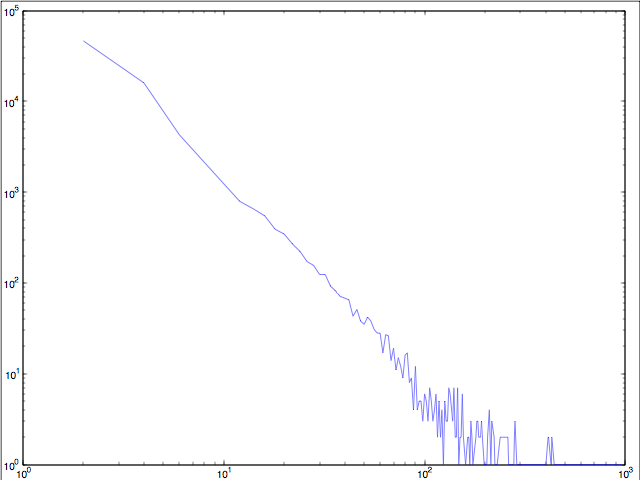
\includegraphics[width=.3\linewidth]{FIG/as-skitter.75000-indd.png}}\hfill
\subfloat[Out-Degree Distribution\label{fig:as-skitter_outdegree}]
  {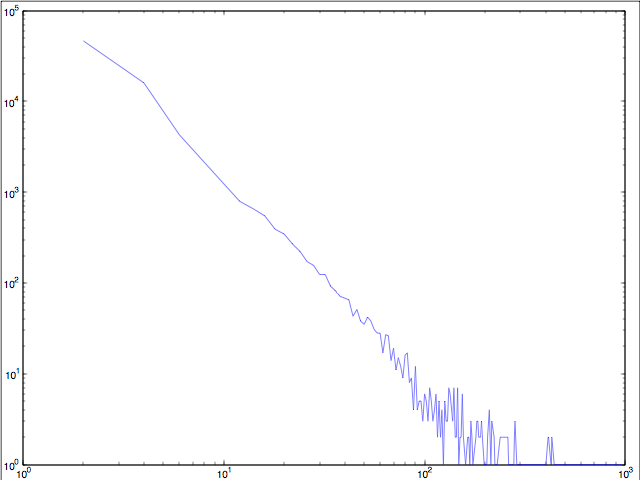
\includegraphics[width=.3\linewidth]{FIG/as-skitter.75000-outdd.png}}\hfill
\subfloat[Degree Distribution\label{fig:as-skitter_degree}]
  {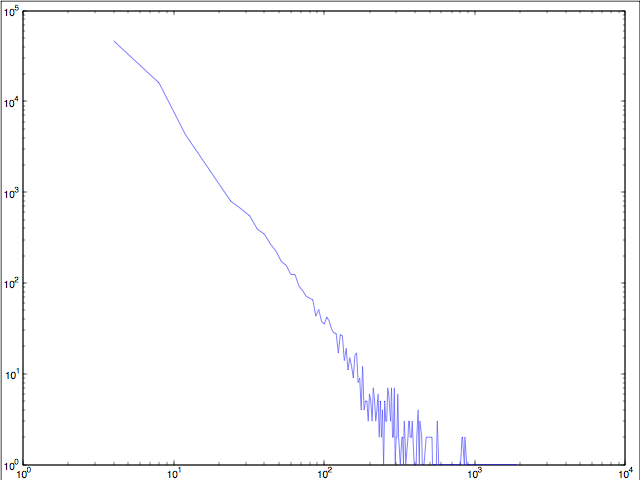
\includegraphics[width=.3\linewidth]{FIG/as-skitter.75000-dd.png}}
\caption{Degree Distributions of as-skitter\label{fig:as-skitter_degree_dist}}
\end{figure}
\begin{figure}
\subfloat[In-Degree Distribution\label{fig:ca-AstroPh_indegree}]
  {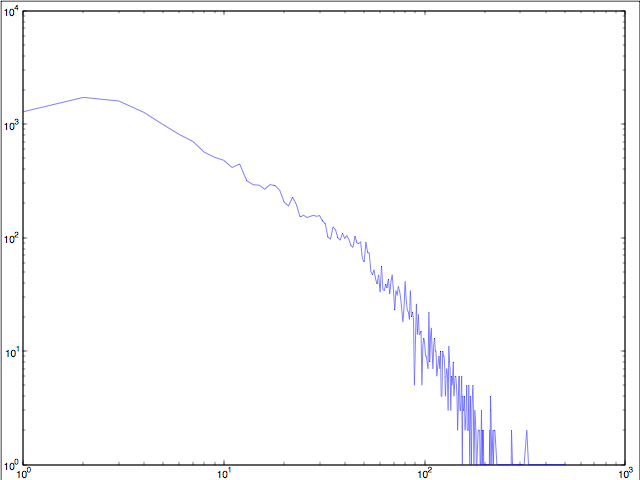
\includegraphics[width=.3\linewidth]{FIG/ca-AstroPh-indd.png}}\hfill
\subfloat[Out-Degree Distribution\label{fig:ca-AstroPh_outdegree}]
  {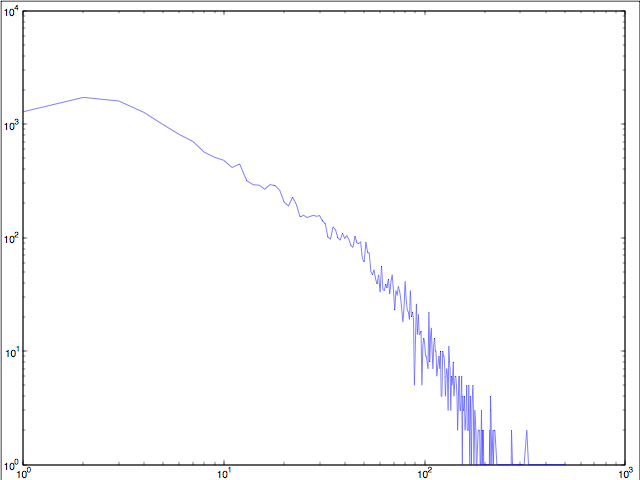
\includegraphics[width=.3\linewidth]{FIG/ca-AstroPh-outdd.png}}\hfill
\subfloat[Degree Distribution\label{fig:ca-AstroPh_degree}]
  {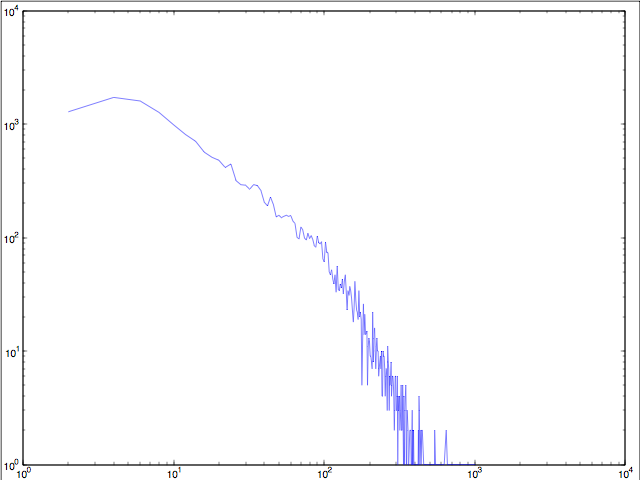
\includegraphics[width=.3\linewidth]{FIG/ca-AstroPh-dd.png}}
\caption{Degree Distributions of a-AstroPh\label{fig:ca-AstroPh_degree_dist}}
\end{figure}
\begin{figure}
\subfloat[In-Degree Distribution\label{fig:cit-HepPh_indegree}]
  {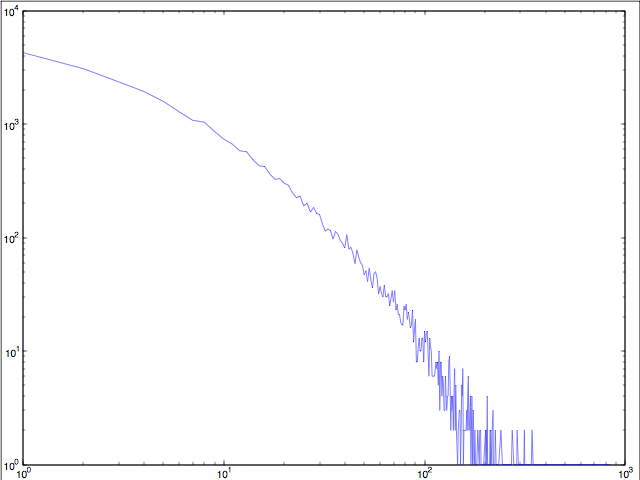
\includegraphics[width=.3\linewidth]{FIG/cit-HepPh-indd.png}}\hfill
\subfloat[Out-Degree Distribution\label{fig:cit-HepPh_outdegree}]
  {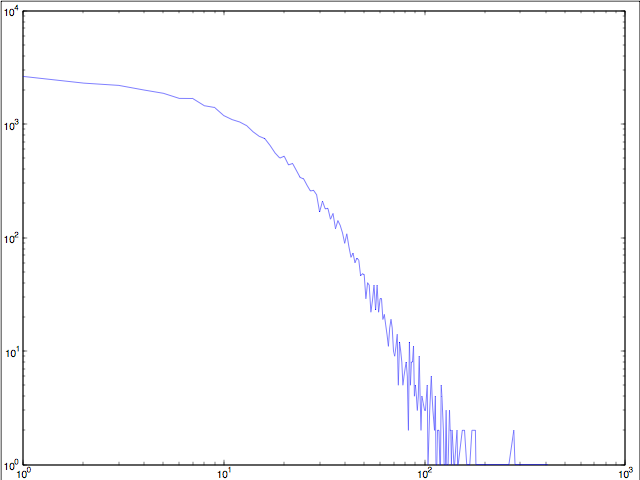
\includegraphics[width=.3\linewidth]{FIG/cit-HepPh-outdd.png}}\hfill
\subfloat[Degree Distribution\label{fig:cit-HepPh_degree}]
  {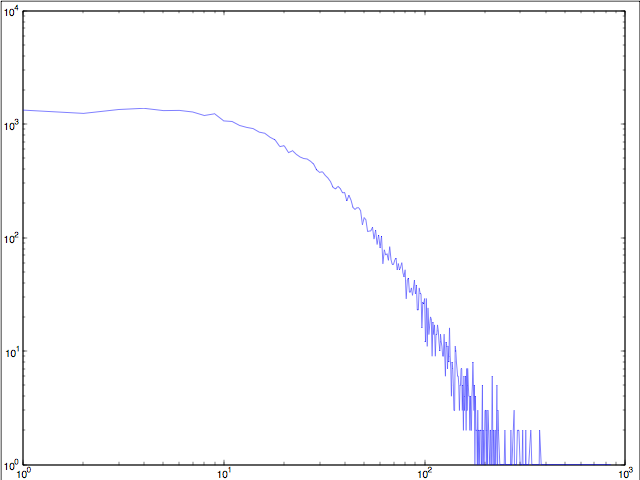
\includegraphics[width=.3\linewidth]{FIG/cit-HepPh-dd.png}}
\caption{Degree Distributions of cit-HepPh\label{fig:cit-HepPh_degree_dist}}
\end{figure}
\begin{figure}
\subfloat[In-Degree Distribution\label{fig:cit-HepTh_indegree}]
  {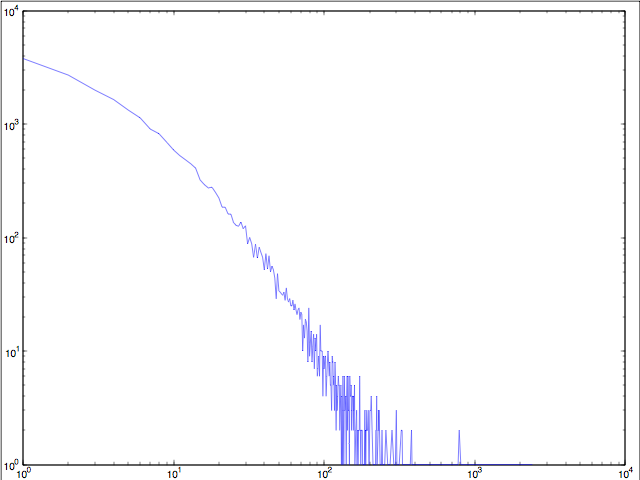
\includegraphics[width=.3\linewidth]{FIG/cit-HepTh-indd.png}}\hfill
\subfloat[Out-Degree Distribution\label{fig:cit-HepTh_outdegree}]
  {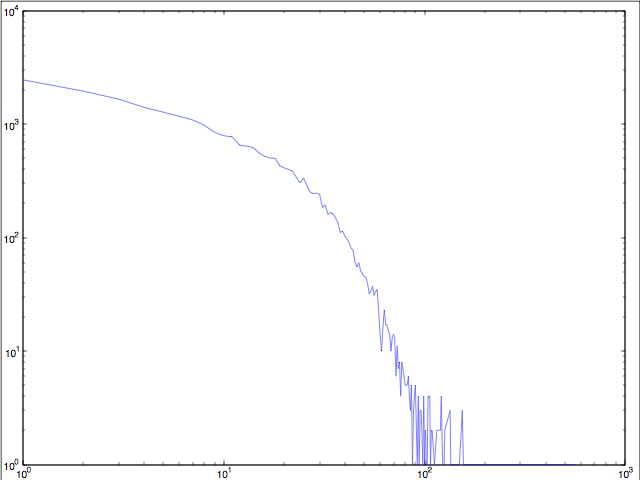
\includegraphics[width=.3\linewidth]{FIG/cit-HepTh-outdd.png}}\hfill
\subfloat[Degree Distribution\label{fig:cit-HepTh_degree}]
  {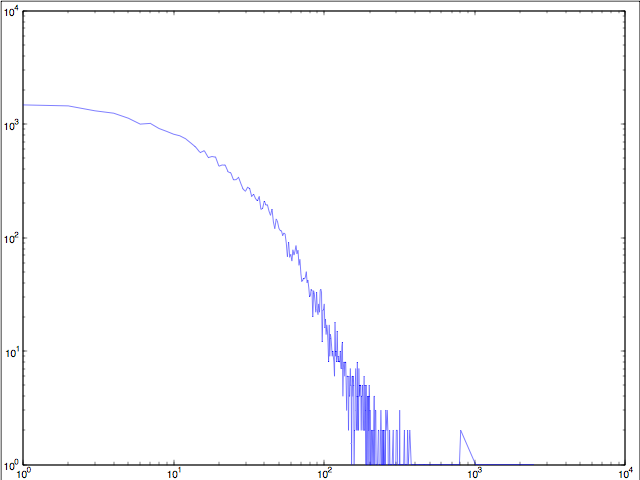
\includegraphics[width=.3\linewidth]{FIG/cit-HepTh-dd.png}}
\caption{Degree Distributions of cit-HepTh\label{fig:cit-HepTh_degree_dist}}
\end{figure}
\begin{figure}
\subfloat[In-Degree Distribution\label{fig:com-amazon.ungraph_indegree}]
  {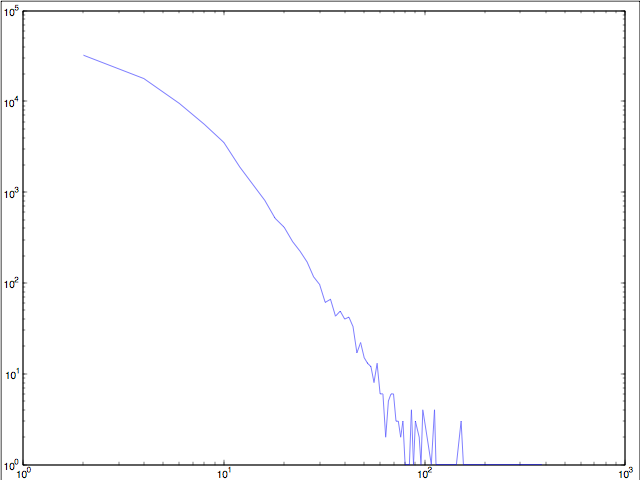
\includegraphics[width=.3\linewidth]{FIG/com-amazon.ungraph-indd.png}}\hfill
\subfloat[Out-Degree Distribution\label{fig:com-amazon.ungraph_outdegree}]
  {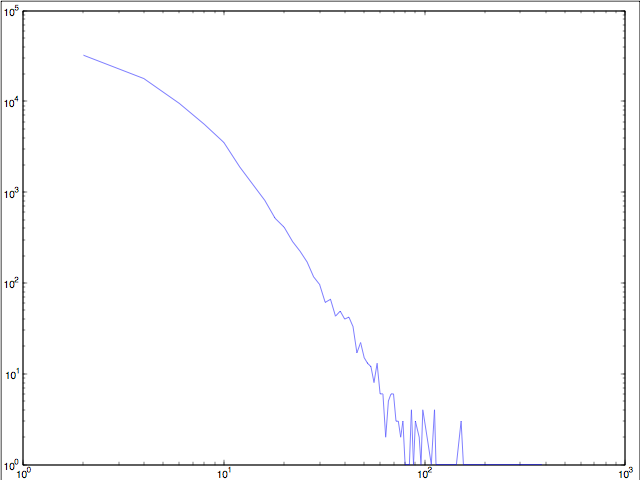
\includegraphics[width=.3\linewidth]{FIG/com-amazon.ungraph-outdd.png}}\hfill
\subfloat[Degree Distribution\label{fig:com-amazon.ungraph_degree}]
  {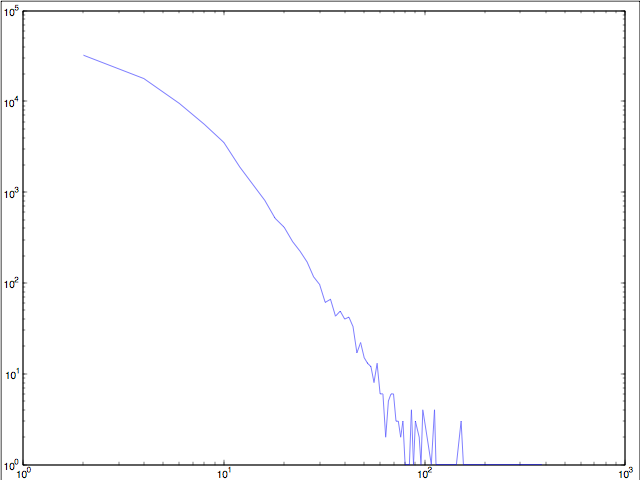
\includegraphics[width=.3\linewidth]{FIG/com-amazon.ungraph-dd.png}}
\caption{Degree Distributions of com-amazon.ungraph\label{fig:com-amazon.ungraph_degree_dist}}
\end{figure}
\begin{figure}
\subfloat[In-Degree Distribution\label{fig:com-dblp.ungraph_indegree}]
  {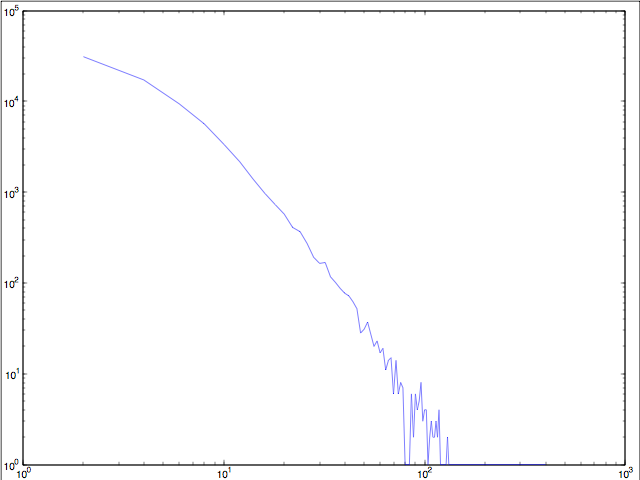
\includegraphics[width=.3\linewidth]{FIG/com-dblp.ungraph-indd.png}}\hfill
\subfloat[Out-Degree Distribution\label{fig:com-dblp.ungraph_outdegree}]
  {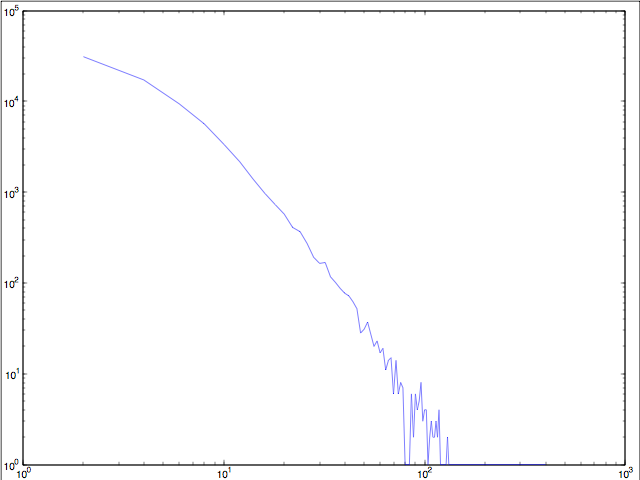
\includegraphics[width=.3\linewidth]{FIG/com-dblp.ungraph-outdd.png}}\hfill
\subfloat[Degree Distribution\label{fig:com-dblp.ungraph_degree}]
  {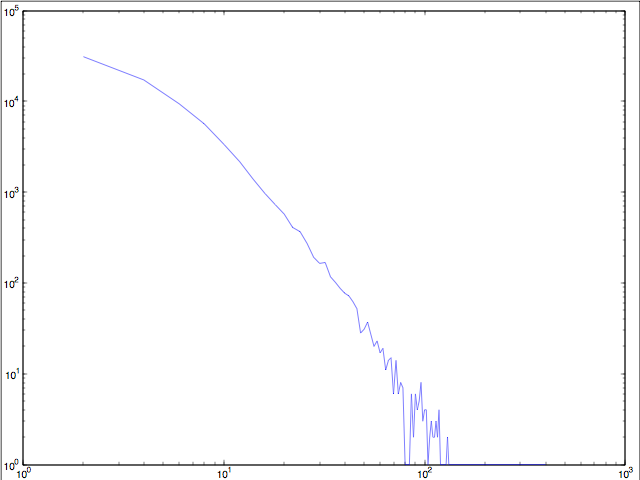
\includegraphics[width=.3\linewidth]{FIG/com-dblp.ungraph-dd.png}}
\caption{Degree Distributions of com-dblp.ungraph\label{fig:com-dblp.ungraph_degree_dist}}
\end{figure}
\begin{figure}
\subfloat[In-Degree Distribution\label{fig:email-Enron.ungraph_indegree}]
  {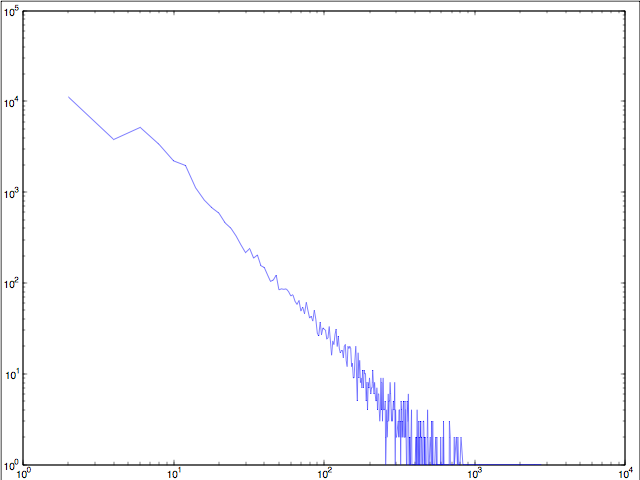
\includegraphics[width=.3\linewidth]{FIG/email-Enron.ungraph-indd.png}}\hfill
\subfloat[Out-Degree Distribution\label{fig:email-Enron.ungraph_outdegree}]
  {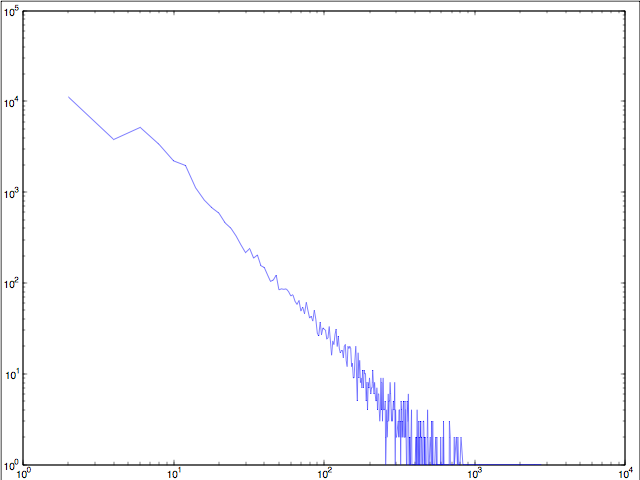
\includegraphics[width=.3\linewidth]{FIG/email-Enron.ungraph-outdd.png}}\hfill
\subfloat[Degree Distribution\label{fig:email-Enron.ungraph_degree}]
  {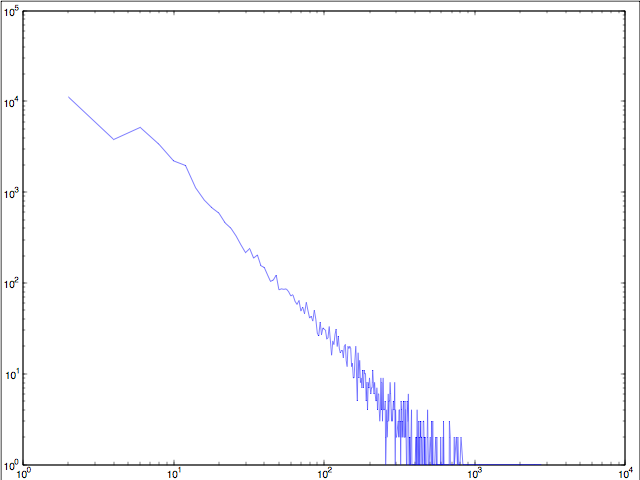
\includegraphics[width=.3\linewidth]{FIG/email-Enron.ungraph-dd.png}}
\caption{Degree Distributions of email-Enron.ungraph\label{fig:email-Enron.ungraph_degree_dist}}
\end{figure}
\begin{figure}
\subfloat[In-Degree Distribution\label{fig:email-EuAll_indegree}]
  {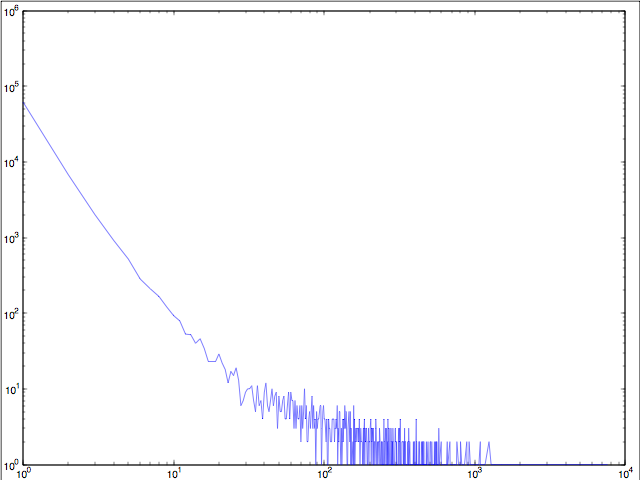
\includegraphics[width=.3\linewidth]{FIG/email-EuAll-indd.png}}\hfill
\subfloat[Out-Degree Distribution\label{fig:email-EuAll_outdegree}]
  {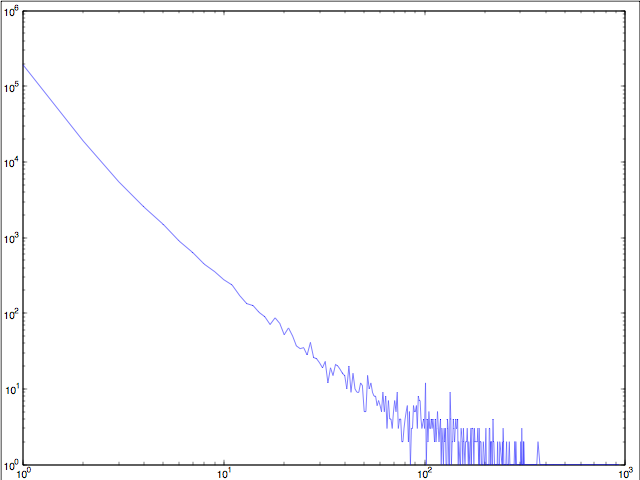
\includegraphics[width=.3\linewidth]{FIG/email-EuAll-outdd.png}}\hfill
\subfloat[Degree Distribution\label{fig:email-EuAll_degree}]
  {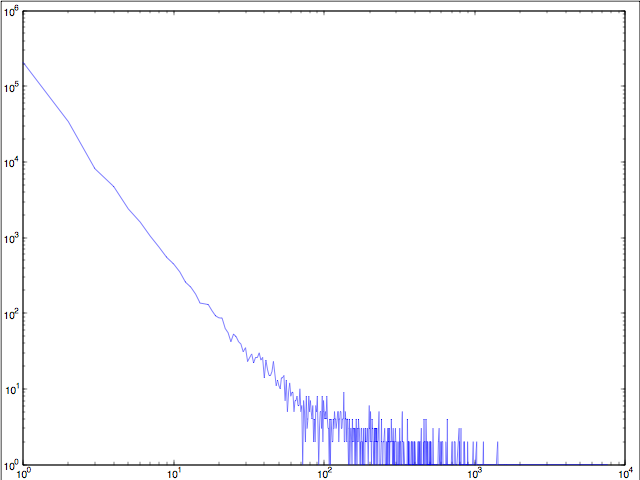
\includegraphics[width=.3\linewidth]{FIG/email-EuAll-dd.png}}
\caption{Degree Distributions of email-EuAll\label{fig:email-EuAll_degree_dist}}
\end{figure}
\begin{figure}
\subfloat[In-Degree Distribution\label{fig:p2p-Gnutella31_indegree}]
  {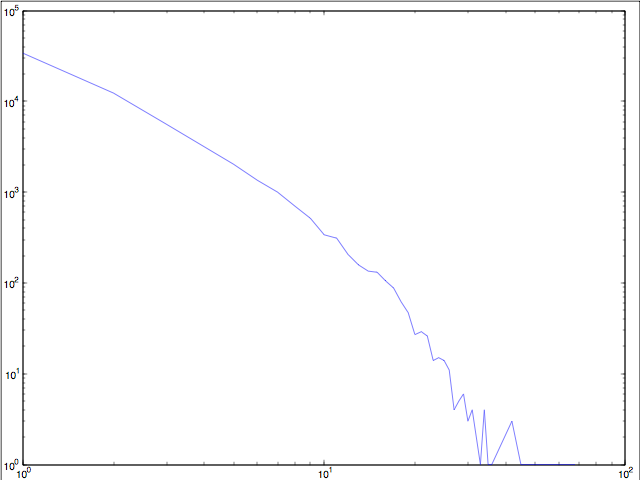
\includegraphics[width=.3\linewidth]{FIG/p2p-Gnutella31-indd.png}}\hfill
\subfloat[Out-Degree Distribution\label{fig:p2p-Gnutella31_outdegree}]
  {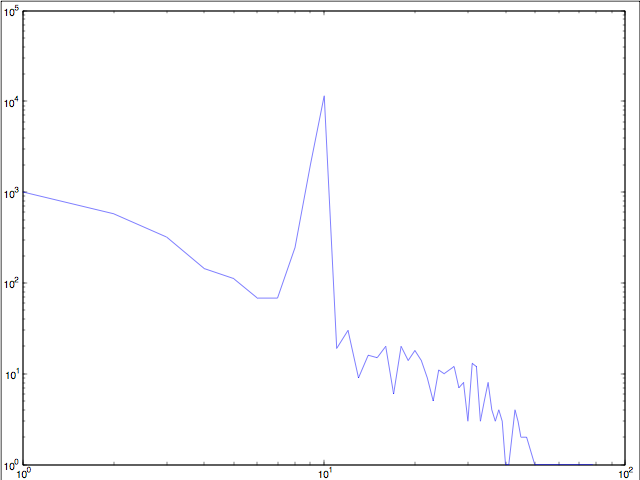
\includegraphics[width=.3\linewidth]{FIG/p2p-Gnutella31-outdd.png}}\hfill
\subfloat[Degree Distribution\label{fig:p2p-Gnutella31_degree}]
  {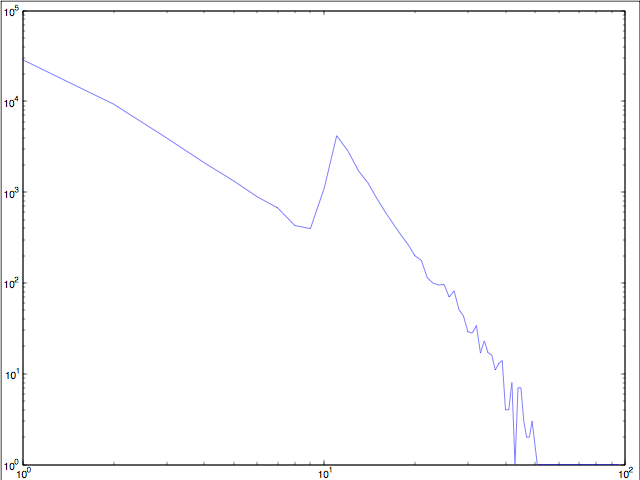
\includegraphics[width=.3\linewidth]{FIG/p2p-Gnutella31-dd.png}}
\caption{Degree Distributions of p2p-Gnutella31\label{fig:p2p-Gnutella31_degree_dist}}
\end{figure}
\begin{figure}
\label{deg_last}
\subfloat[In-Degree Distribution\label{fig:soc-Slashdot0811_indegree}]
  {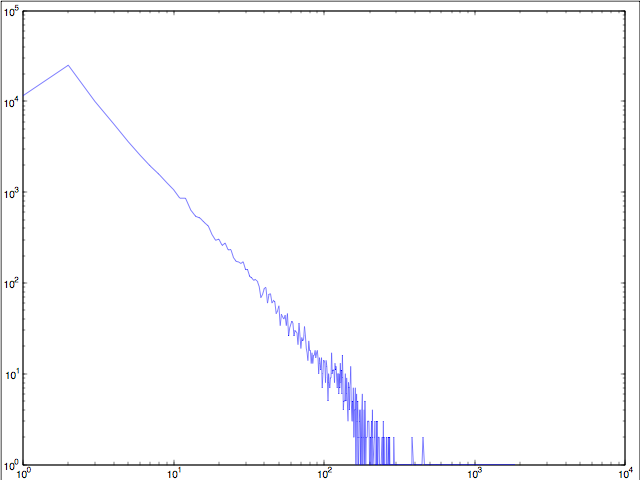
\includegraphics[width=.3\linewidth]{FIG/soc-Slashdot0811-indd.png}}\hfill
\subfloat[Out-Degree Distribution\label{fig:soc-Slashdot0811_outdegree}]
  {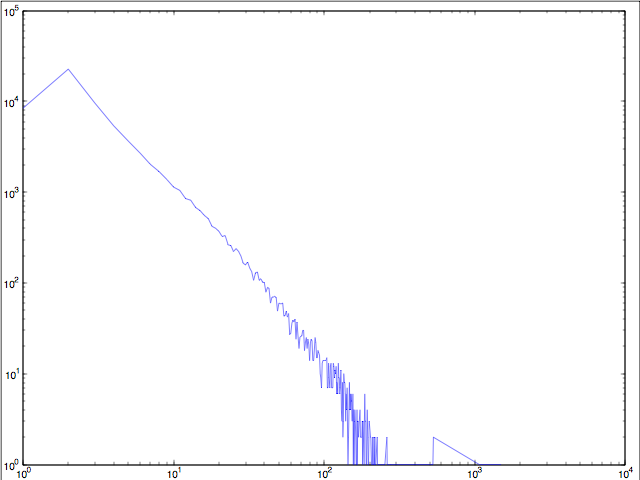
\includegraphics[width=.3\linewidth]{FIG/soc-Slashdot0811-outdd.png}}\hfill
\subfloat[Degree Distribution\label{fig:soc-Slashdot0811_degree}]
  {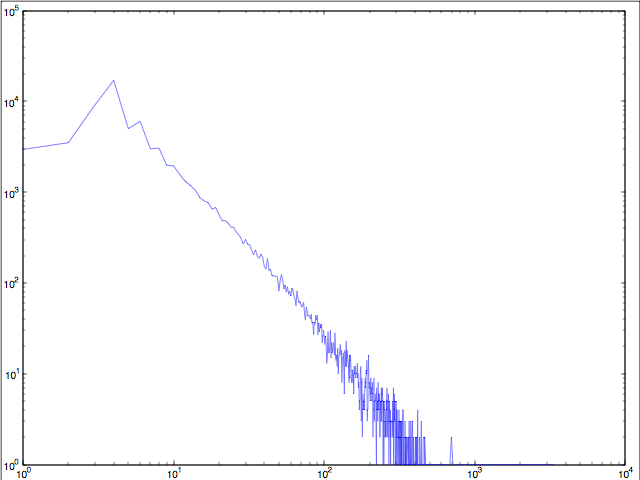
\includegraphics[width=.3\linewidth]{FIG/soc-Slashdot0811-dd.png}}
\caption{Degree Distributions of soc-Slashdot0811\label{fig:soc-Slashdot0811_degree_dist}}
\end{figure}
\begin{figure}
\subfloat[In-Degree Distribution\label{fig:as-Caida.undir_indegree}]
  {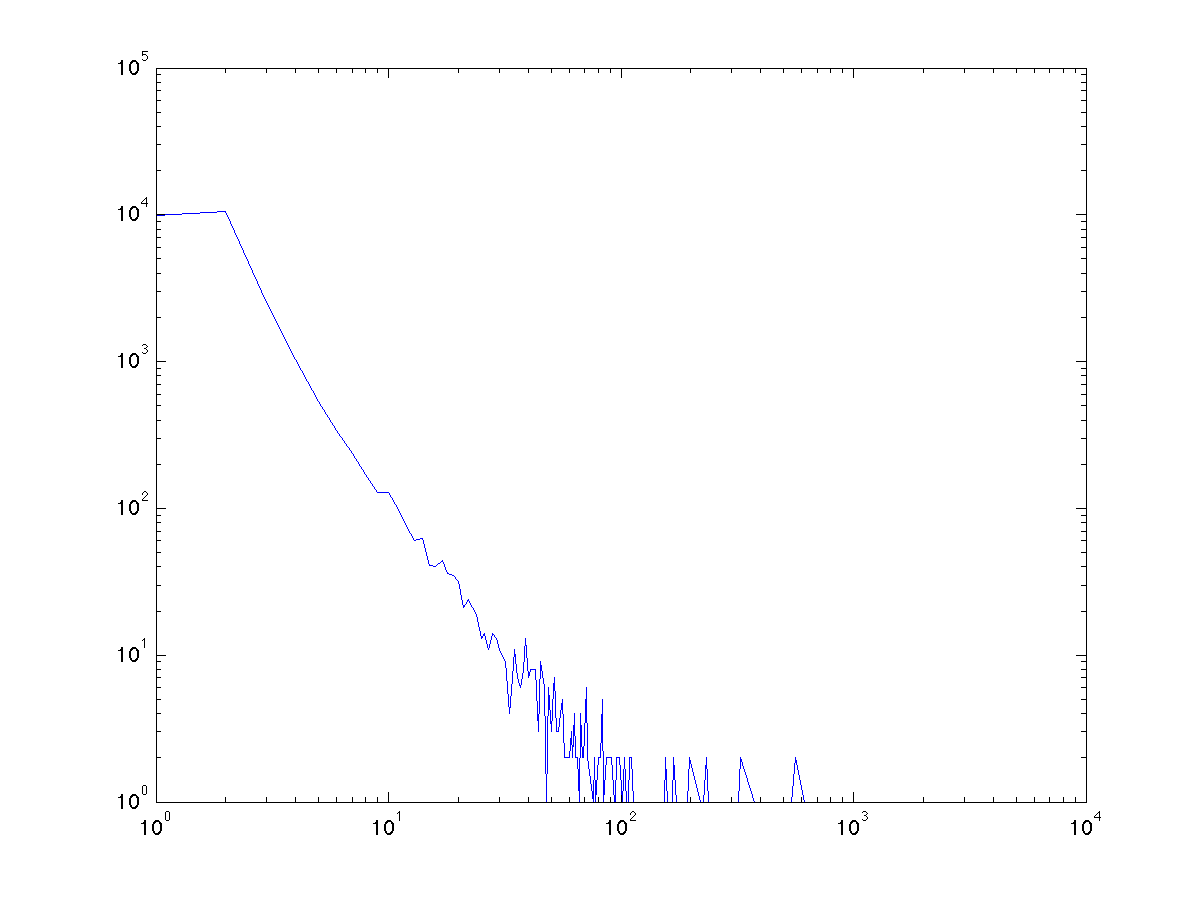
\includegraphics[width=.3\linewidth]{FIG/as-Caida.undir.txt-indegreedist.png}}\hfill
\subfloat[Out-Degree Distribution\label{fig:as-Caida.undir_outdegree}]
  {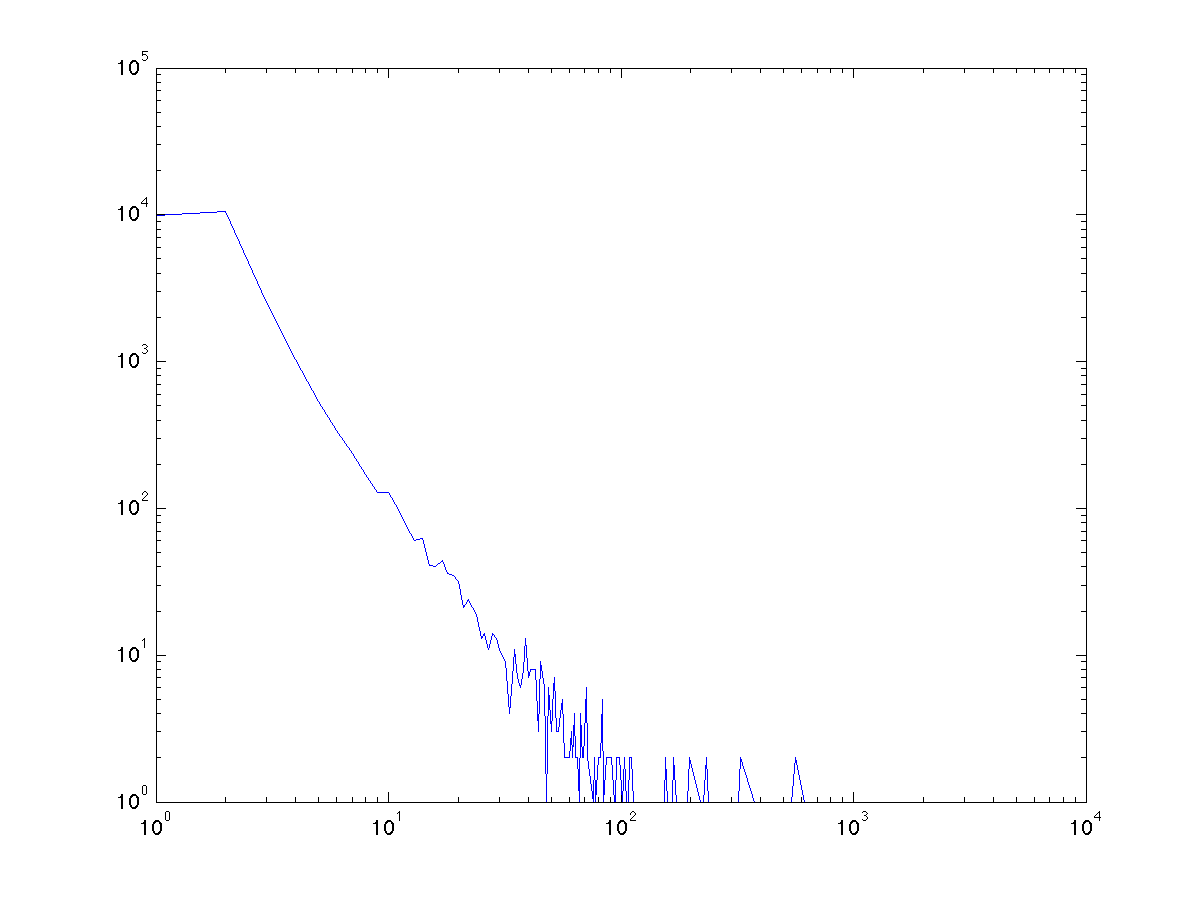
\includegraphics[width=.3\linewidth]{FIG/as-Caida.undir.txt-outdegreedist.png}}\hfill
\subfloat[Degree Distribution\label{fig:as-Caida.undir_degree}]
  {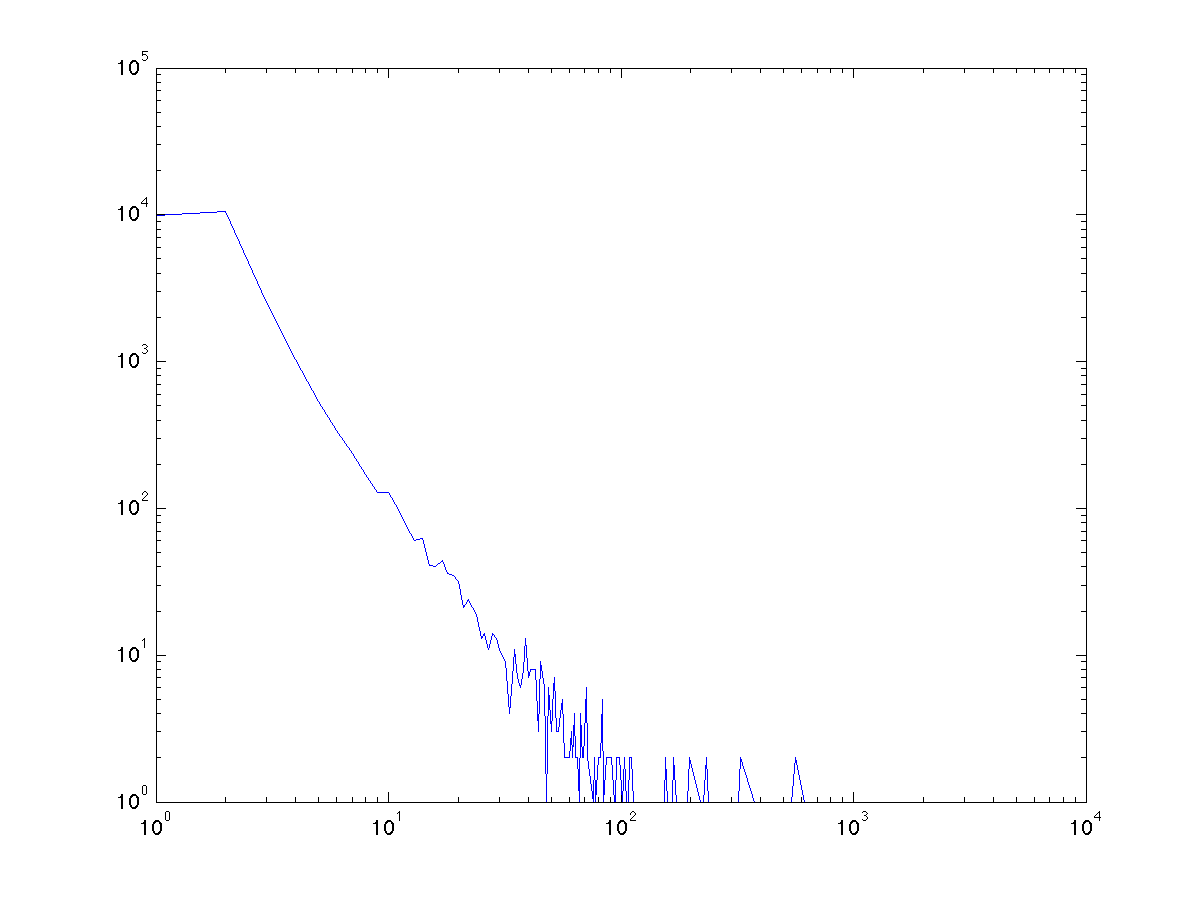
\includegraphics[width=.3\linewidth]{FIG/as-Caida.undir.txt-degree.png}}
\caption{Degree Distributions of as-Caida\label{fig:as-Caida.undir.txt_degree_dist}}
\end{figure}
\begin{figure}
\subfloat[In-Degree Distribution\label{fig:bio-protein_indegree}]
  {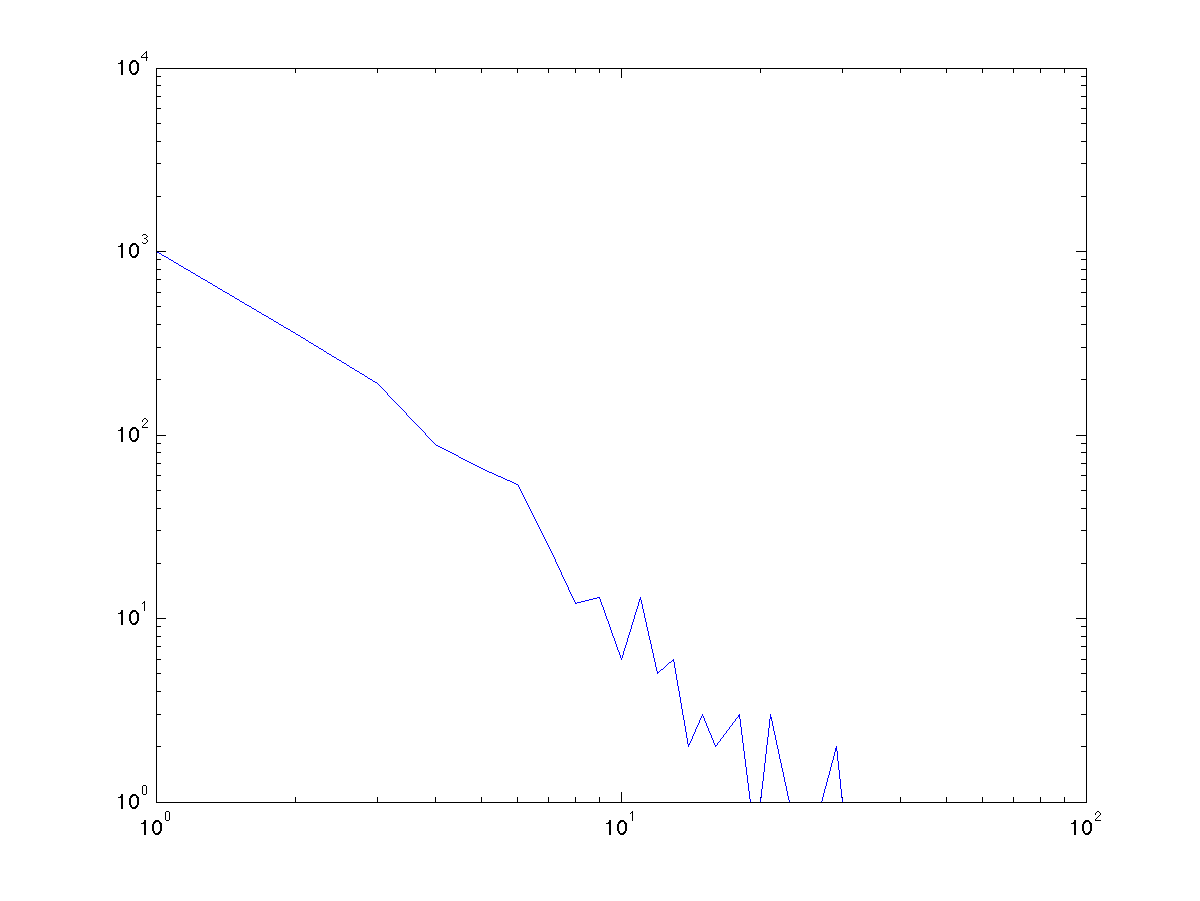
\includegraphics[width=.3\linewidth]{FIG/bio-protein-undir.txt-indegreedist.png}}\hfill
\subfloat[Out-Degree Distribution\label{fig:bio-protein_outdegree}]
  {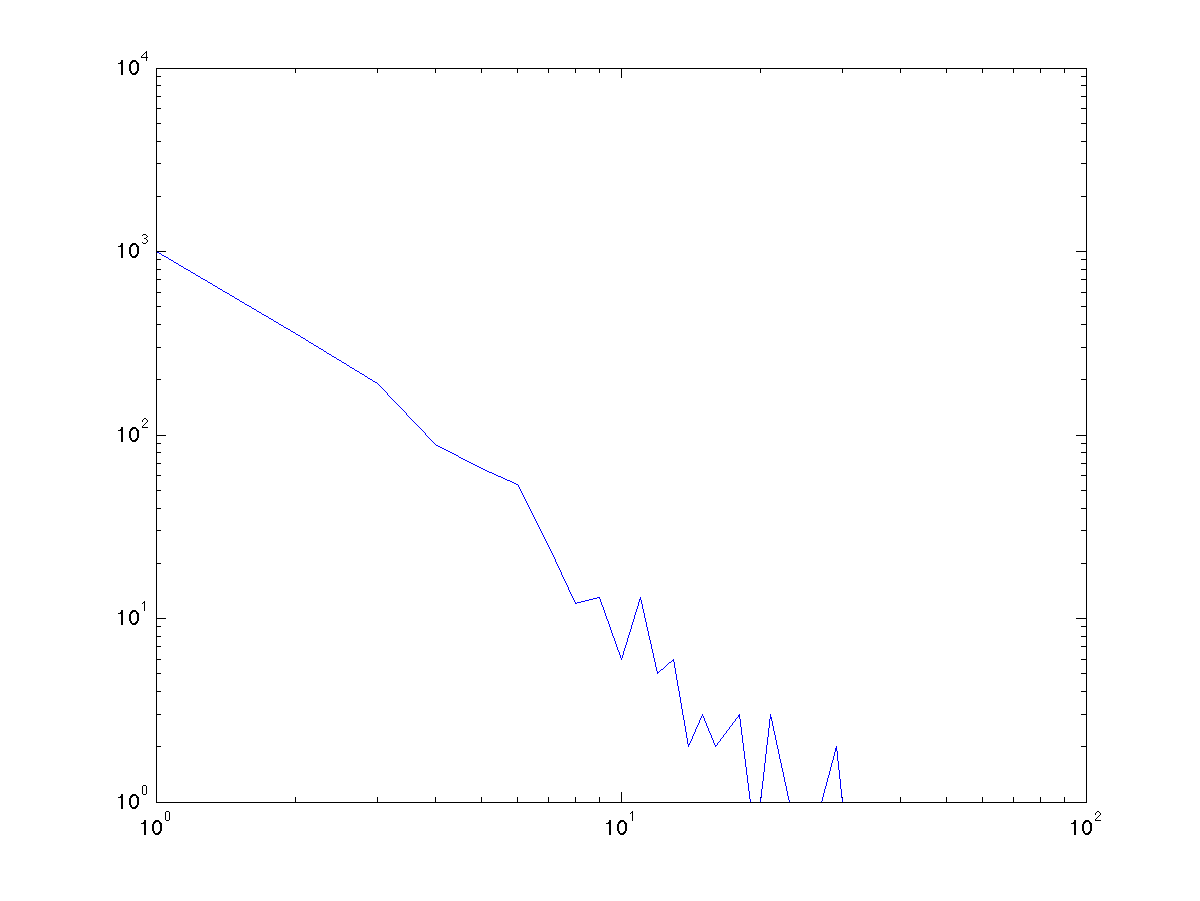
\includegraphics[width=.3\linewidth]{FIG/bio-protein-undir.txt-outdegreedist.png}}\hfill
\subfloat[Degree Distribution\label{fig:bio-protein_degree}]
  {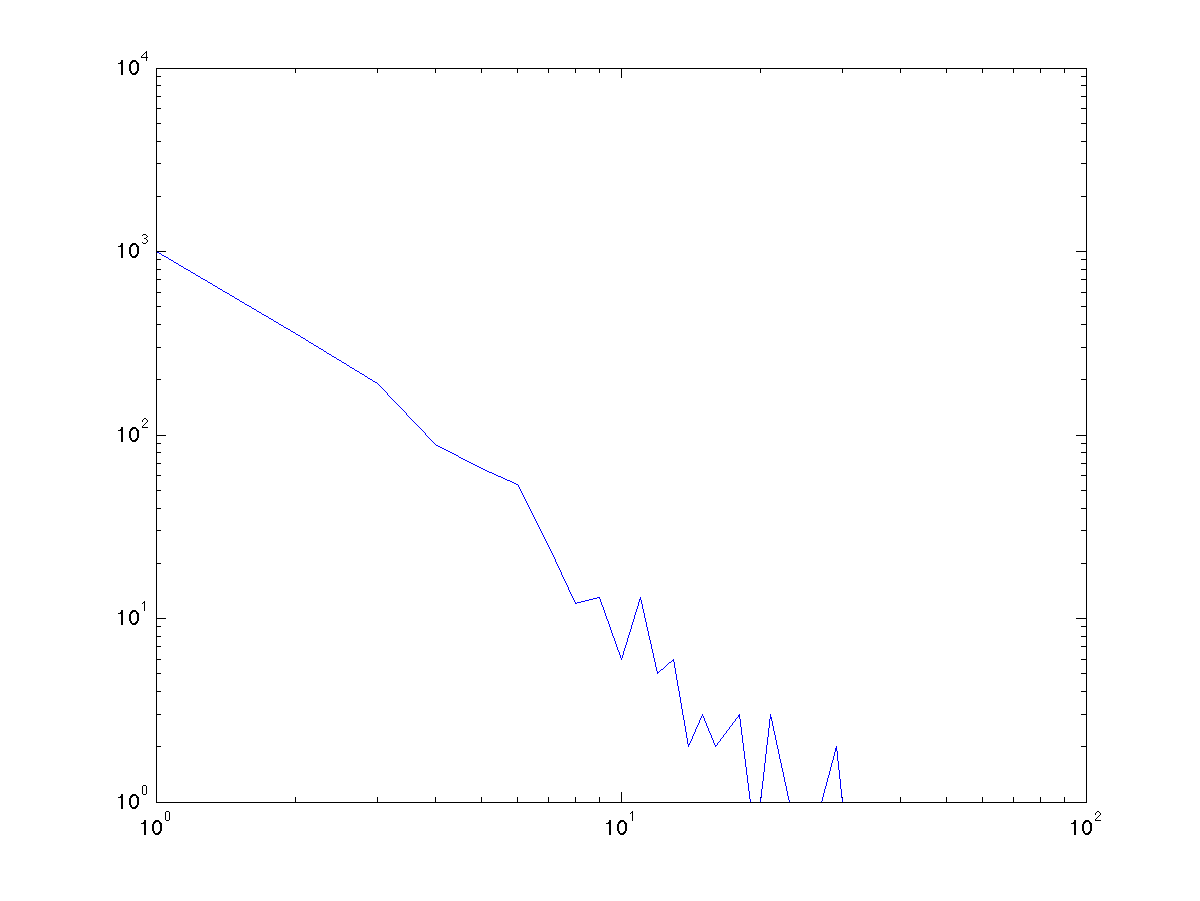
\includegraphics[width=.3\linewidth]{FIG/bio-protein-undir.txt-degree.png}}
\caption{Degree Distributions of bio-protein\label{fig:bio-protein_degree_dist}}
\end{figure}
\begin{figure}
\subfloat[In-Degree Distribution\label{fig:cit-Cora_indegree}]
  {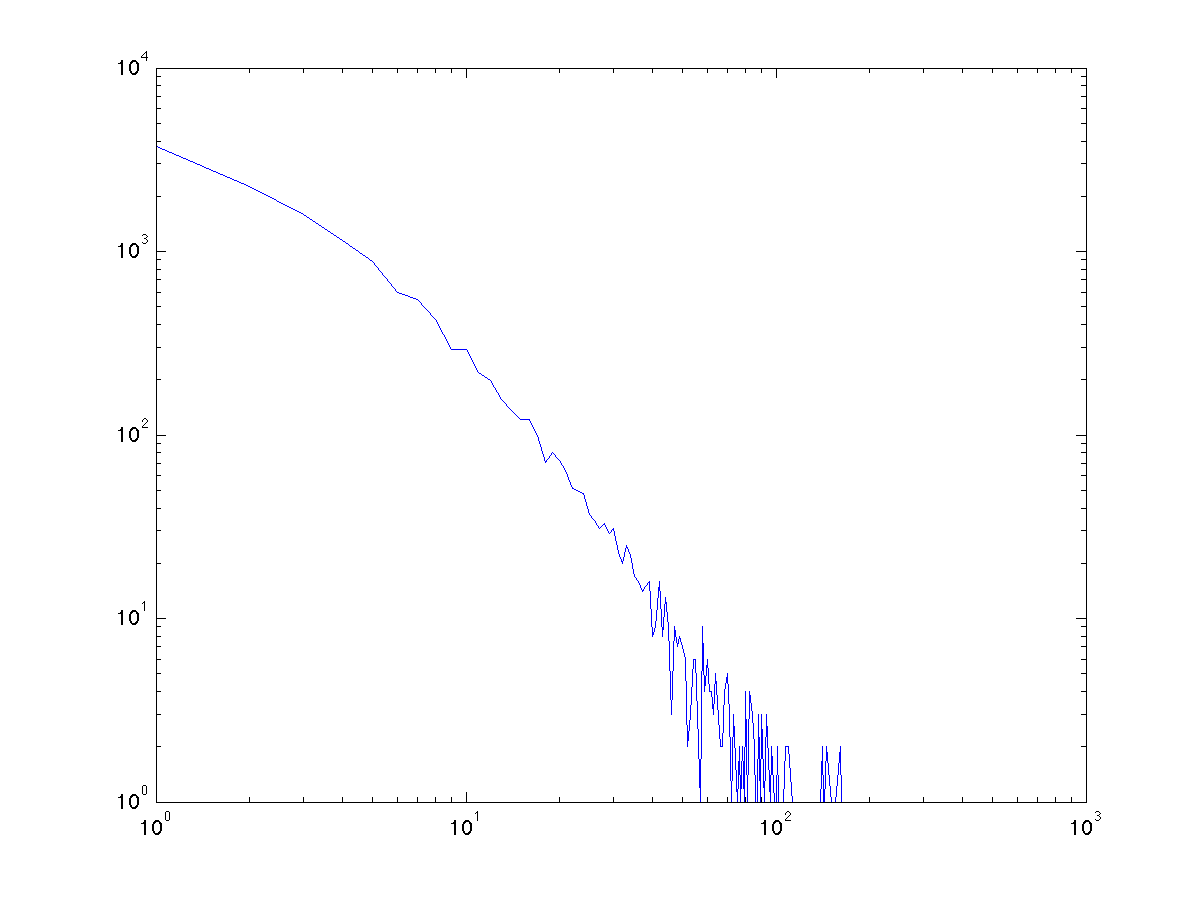
\includegraphics[width=.3\linewidth]{FIG/cit-Cora.txt-indegreedist.png}}\hfill
\subfloat[Out-Degree Distribution\label{fig:cit-Cora_outdegree}]
  {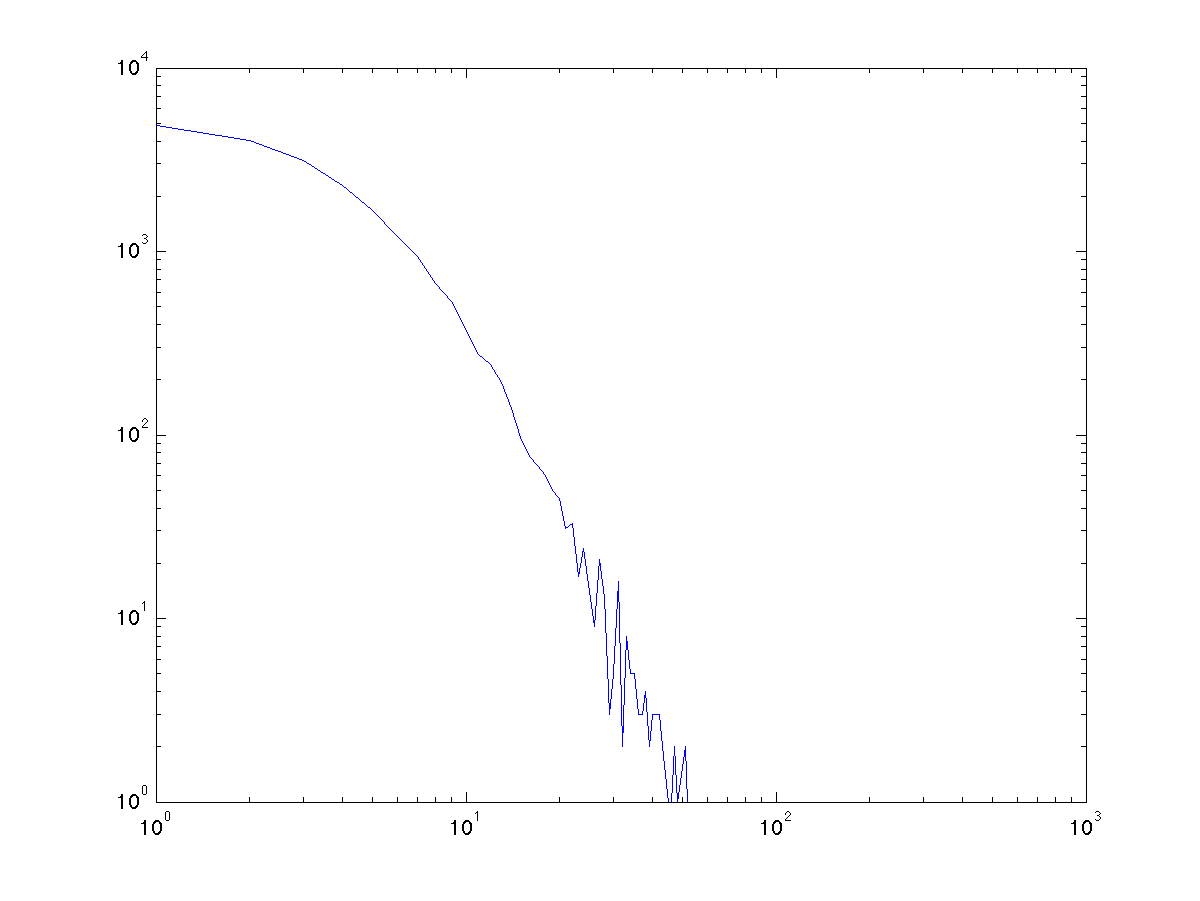
\includegraphics[width=.3\linewidth]{FIG/cit-Cora.txt-outdegreedist.png}}\hfill
\subfloat[Degree Distribution\label{fig:cit-Cora_degree}]
  {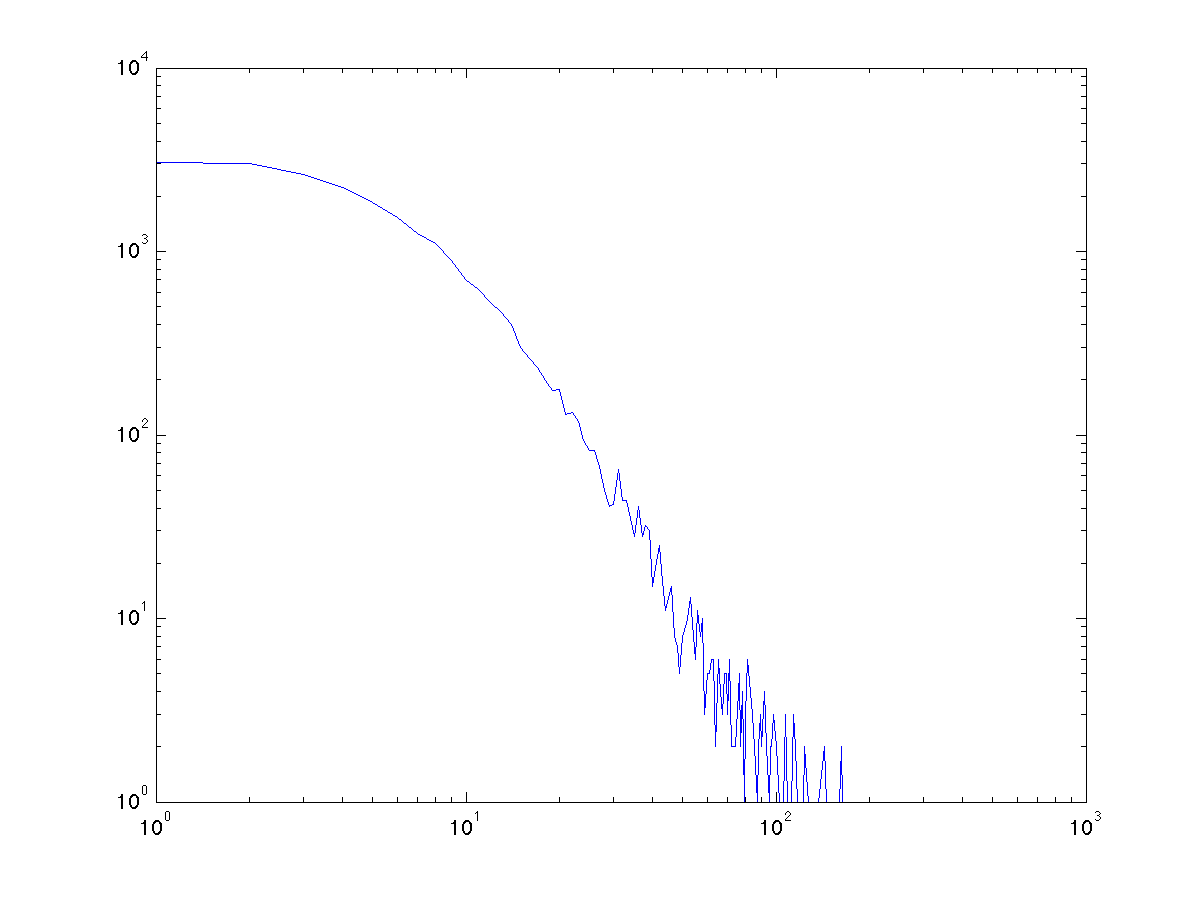
\includegraphics[width=.3\linewidth]{FIG/cit-Cora.txt-degree.png}}
\caption{Degree Distributions of cit-Cora\label{fig:cit-Cora_degree_dist}}
\end{figure}
\begin{figure}
\subfloat[In-Degree Distribution\label{fig:soc-digg_indegree}]
  {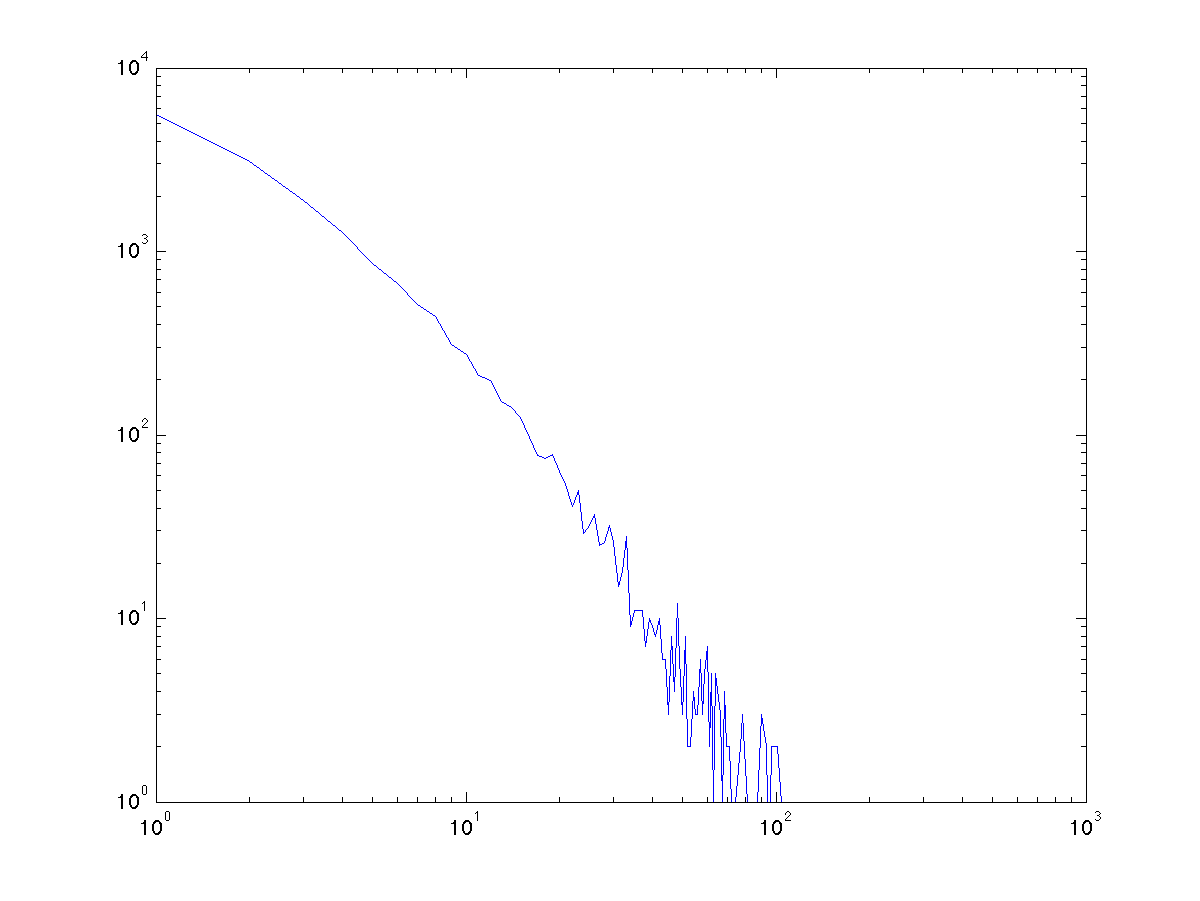
\includegraphics[width=.3\linewidth]{FIG/soc-digg.txt-indegreedist.png}}\hfill
\subfloat[Out-Degree Distribution\label{fig:soc-digg_outdegree}]
  {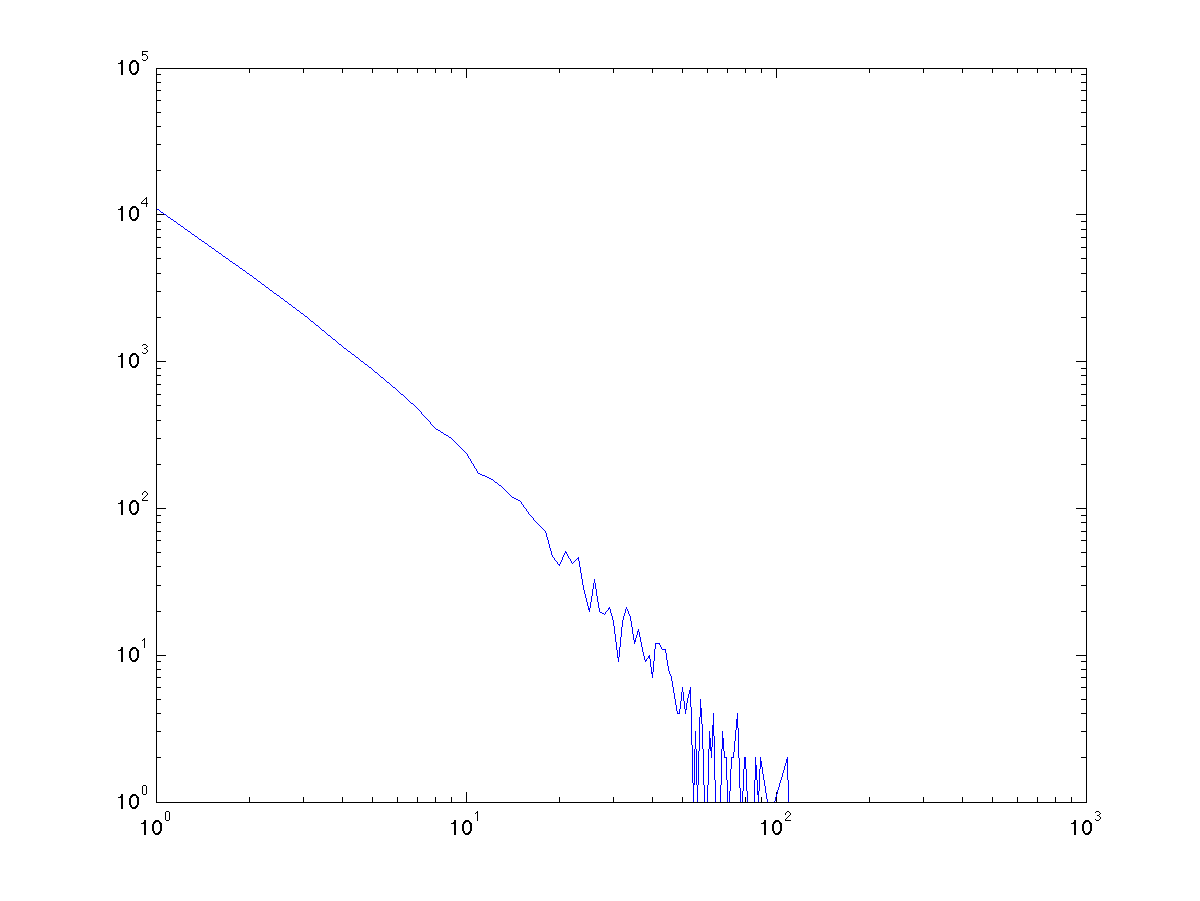
\includegraphics[width=.3\linewidth]{FIG/soc-digg.txt-outdegreedist.png}}\hfill
\subfloat[Degree Distribution\label{fig:soc-digg_degree}]
  {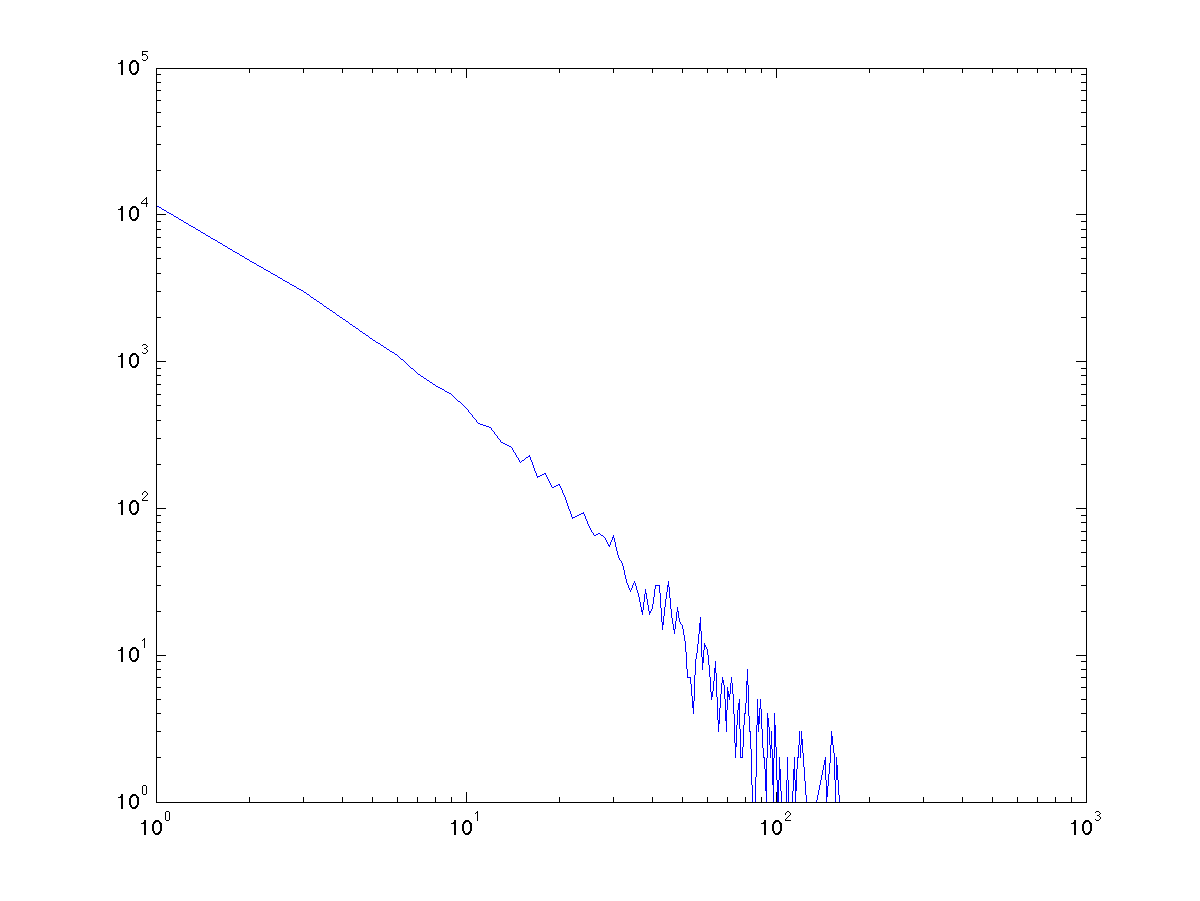
\includegraphics[width=.3\linewidth]{FIG/soc-digg.txt-degree.png}}
\caption{Degree Distributions of soc-digg\label{fig:soc-digg_degree_dist}}
\end{figure}
\begin{figure}
\subfloat[In-Degree Distribution\label{fig:soc-flickr_indegree}]
  {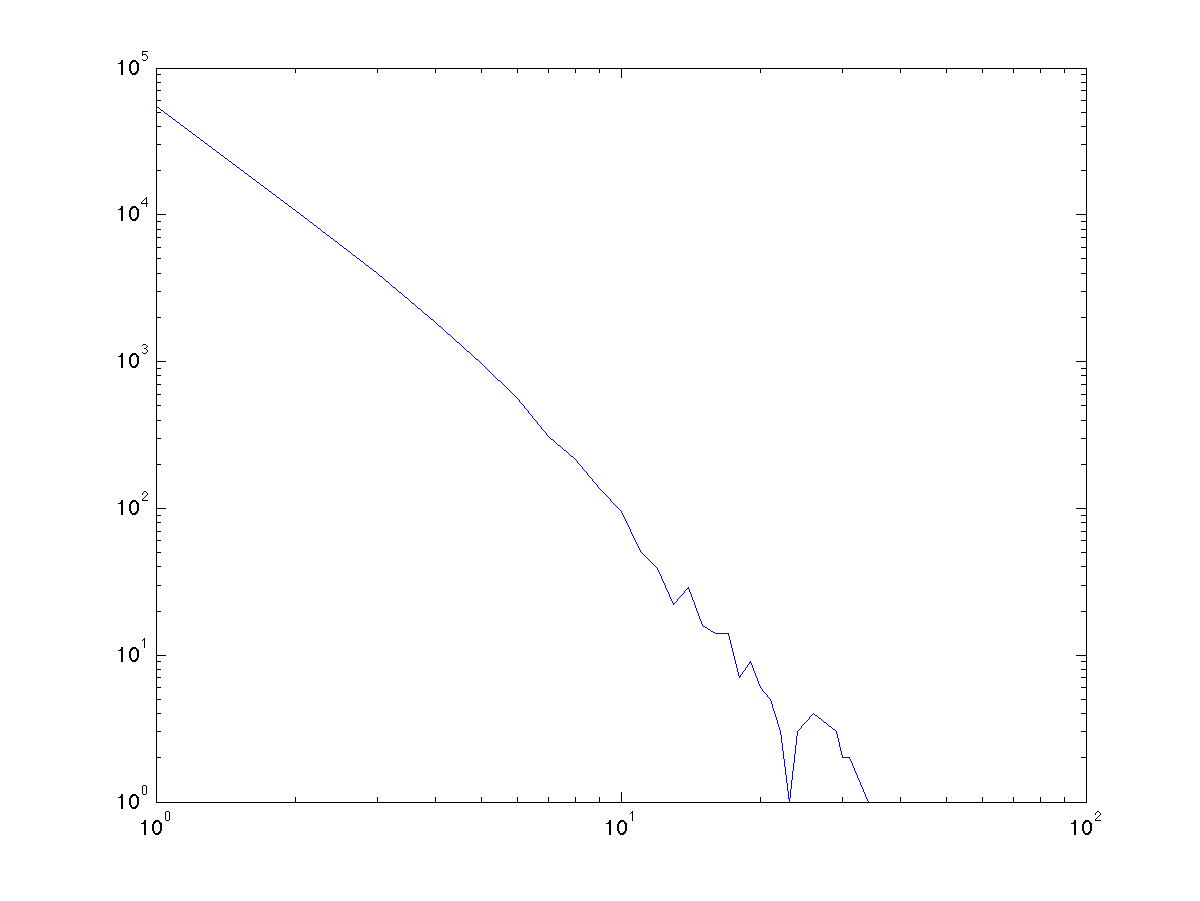
\includegraphics[width=.3\linewidth]{FIG/soc-flickr-75000.txt-indegreedist.png}}\hfill
\subfloat[Out-Degree Distribution\label{fig:soc-flickr_outdegree}]
  {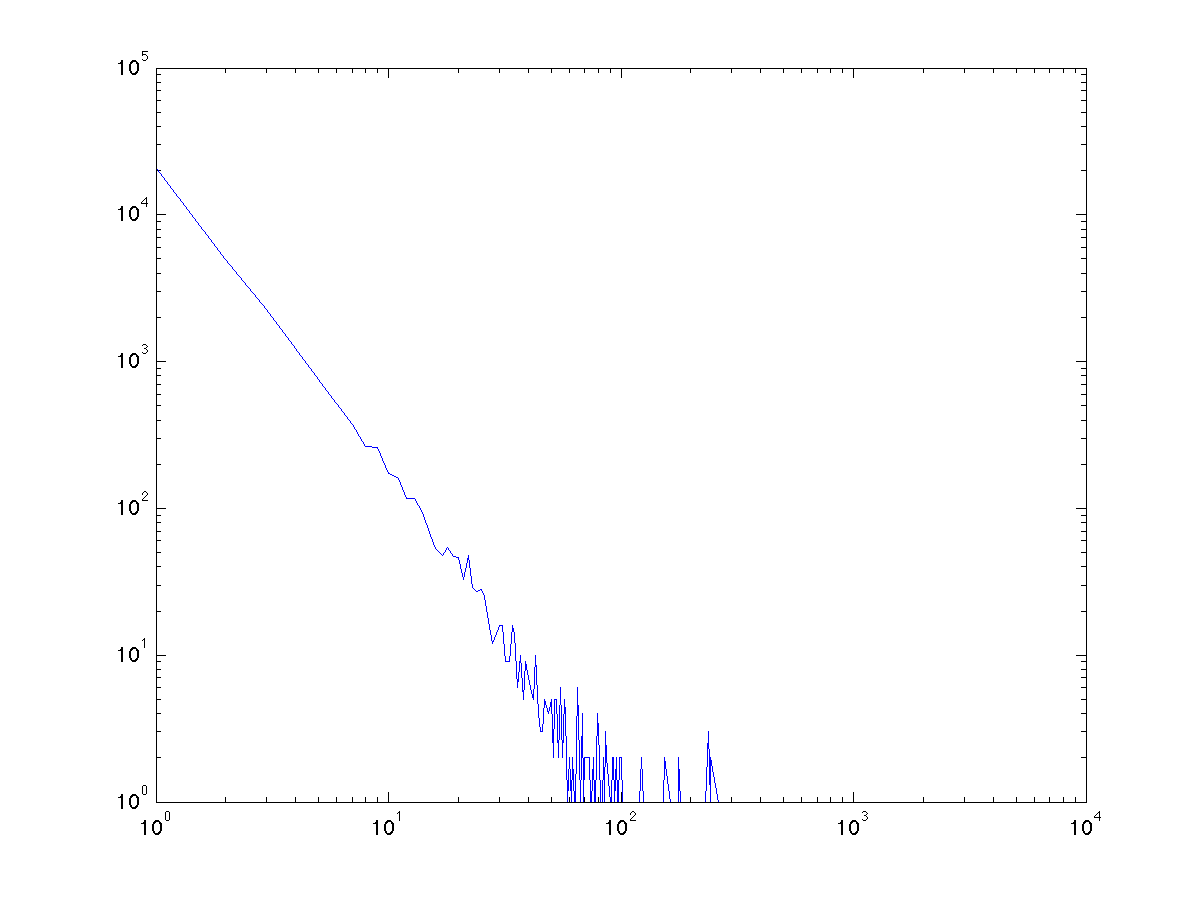
\includegraphics[width=.3\linewidth]{FIG/soc-flickr-75000.txt-outdegreedist.png}}\hfill
\subfloat[Degree Distribution\label{fig:soc-flickr_degree}]
  {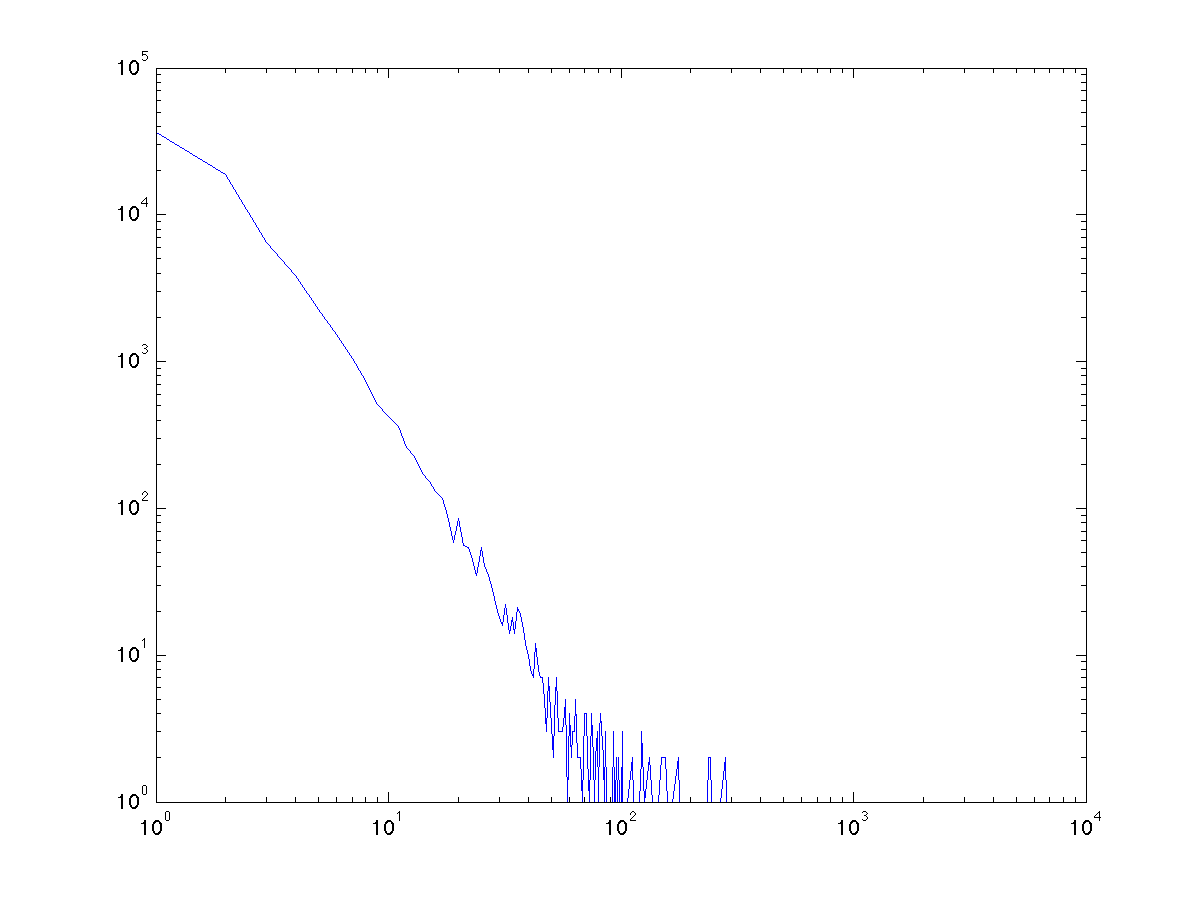
\includegraphics[width=.3\linewidth]{FIG/soc-flickr-75000.txt-degree.png}}
\caption{Degree Distributions of soc-flickr\label{fig:soc-flickr_degree_dist}}
\end{figure}
\begin{figure}
\subfloat[In-Degree Distribution\label{fig:soc-hamsterster_indegree}]
  {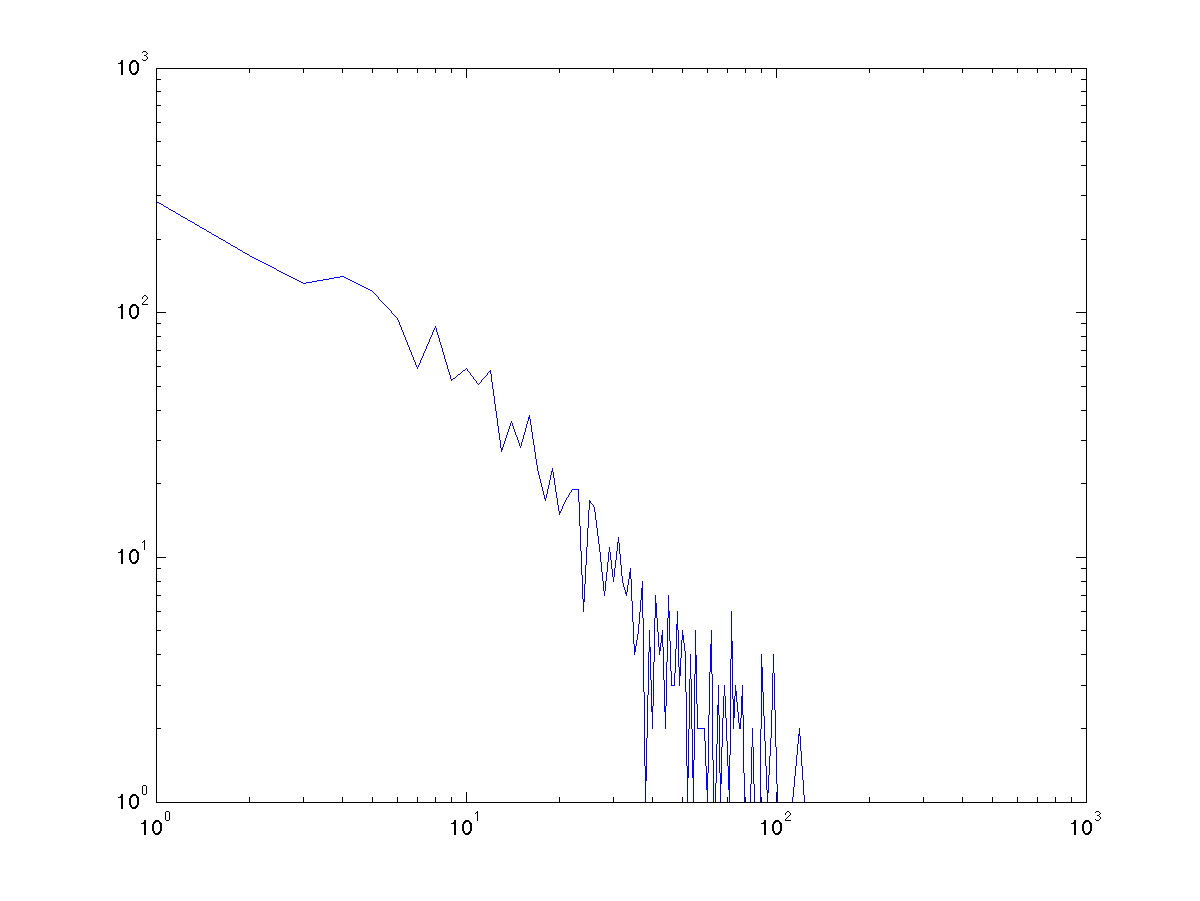
\includegraphics[width=.3\linewidth]{FIG/soc-hamsterster.undir.txt-indegreedist.png}}\hfill
\subfloat[Out-Degree Distribution\label{fig:soc-hamsterster_outdegree}]
  {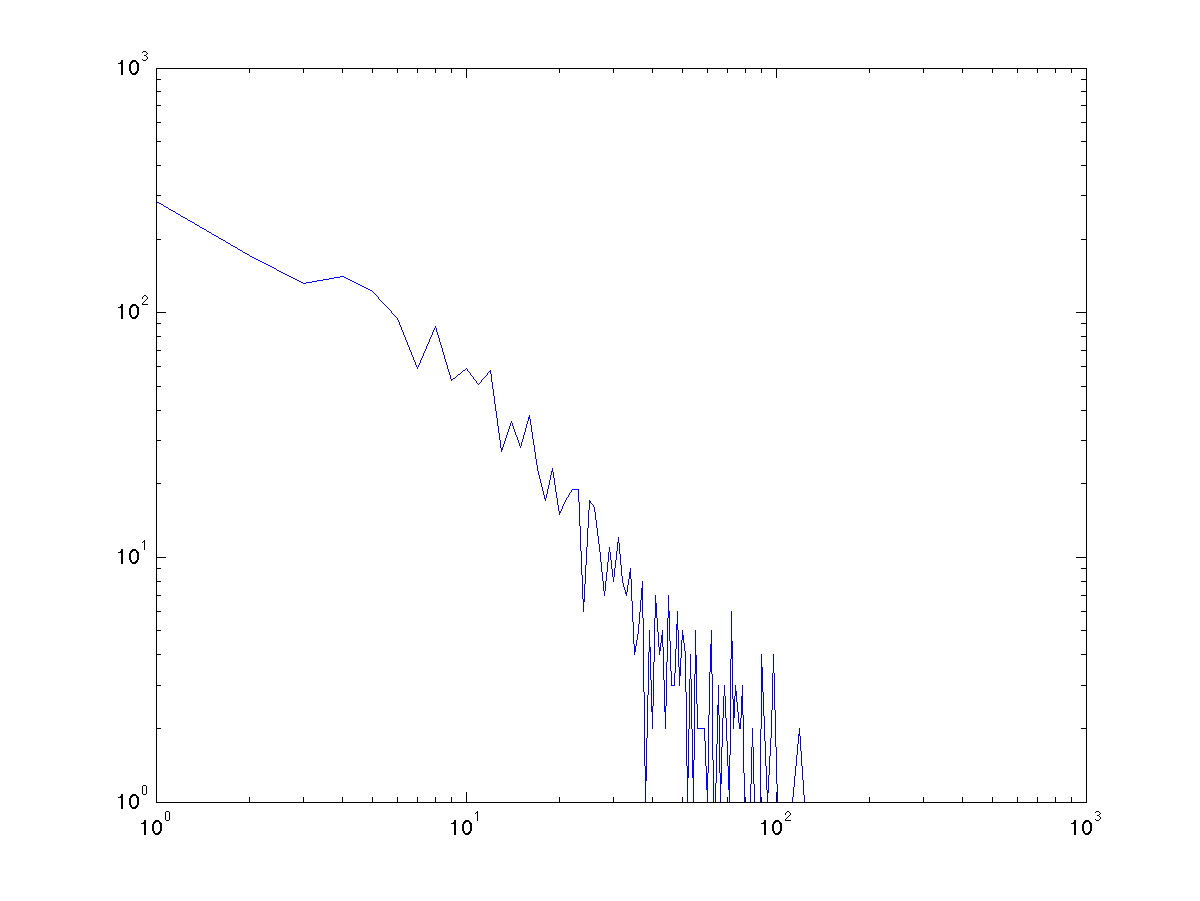
\includegraphics[width=.3\linewidth]{FIG/soc-hamsterster.undir.txt-outdegreedist.png}}\hfill
\subfloat[Degree Distribution\label{fig:soc-hamsterster_degree}]
  {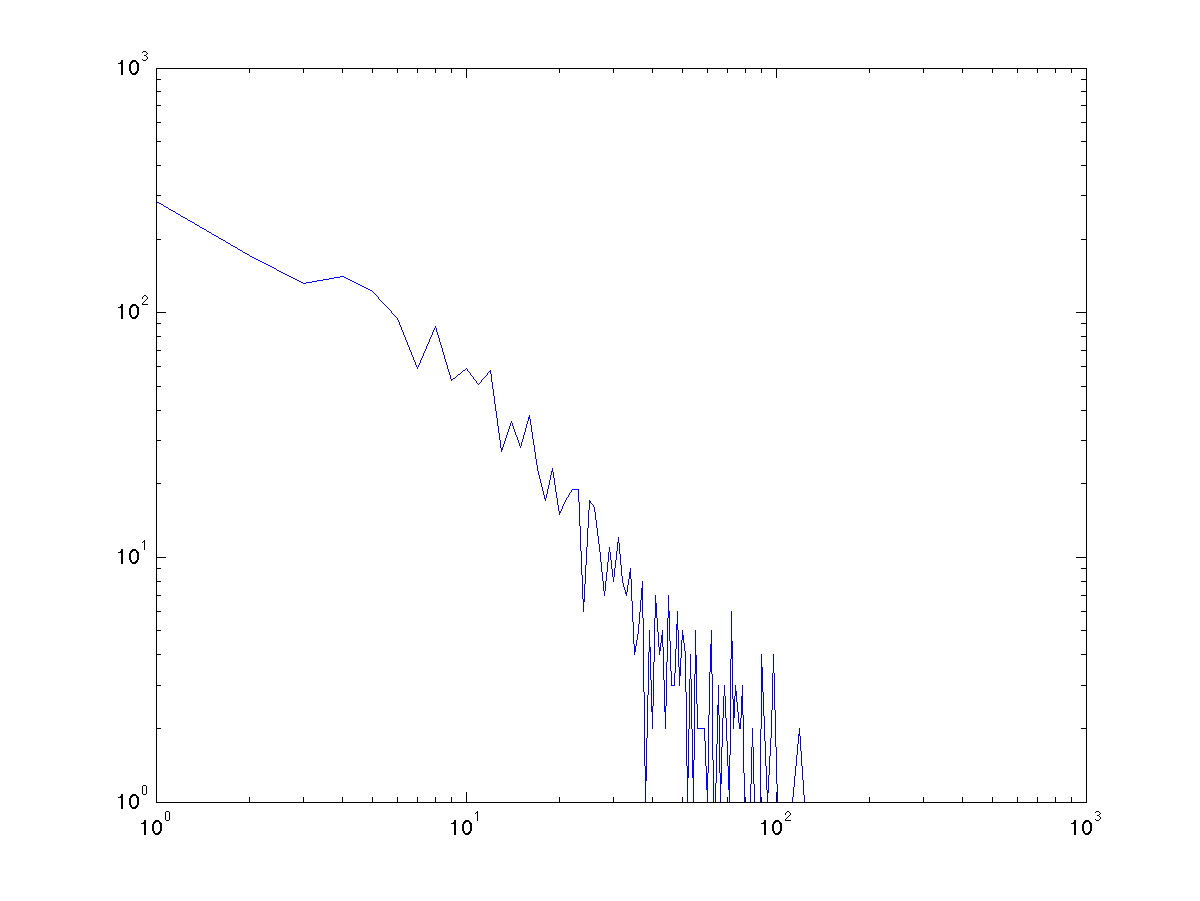
\includegraphics[width=.3\linewidth]{FIG/soc-hamsterster.undir.txt-degree.png}}
\caption{Degree Distributions of soc-hamsterster\label{fig:soc-hamsterster_degree_dist}}
\end{figure}
\begin{figure}
\subfloat[In-Degree Distribution\label{fig:soc-pokec_indegree}]
  {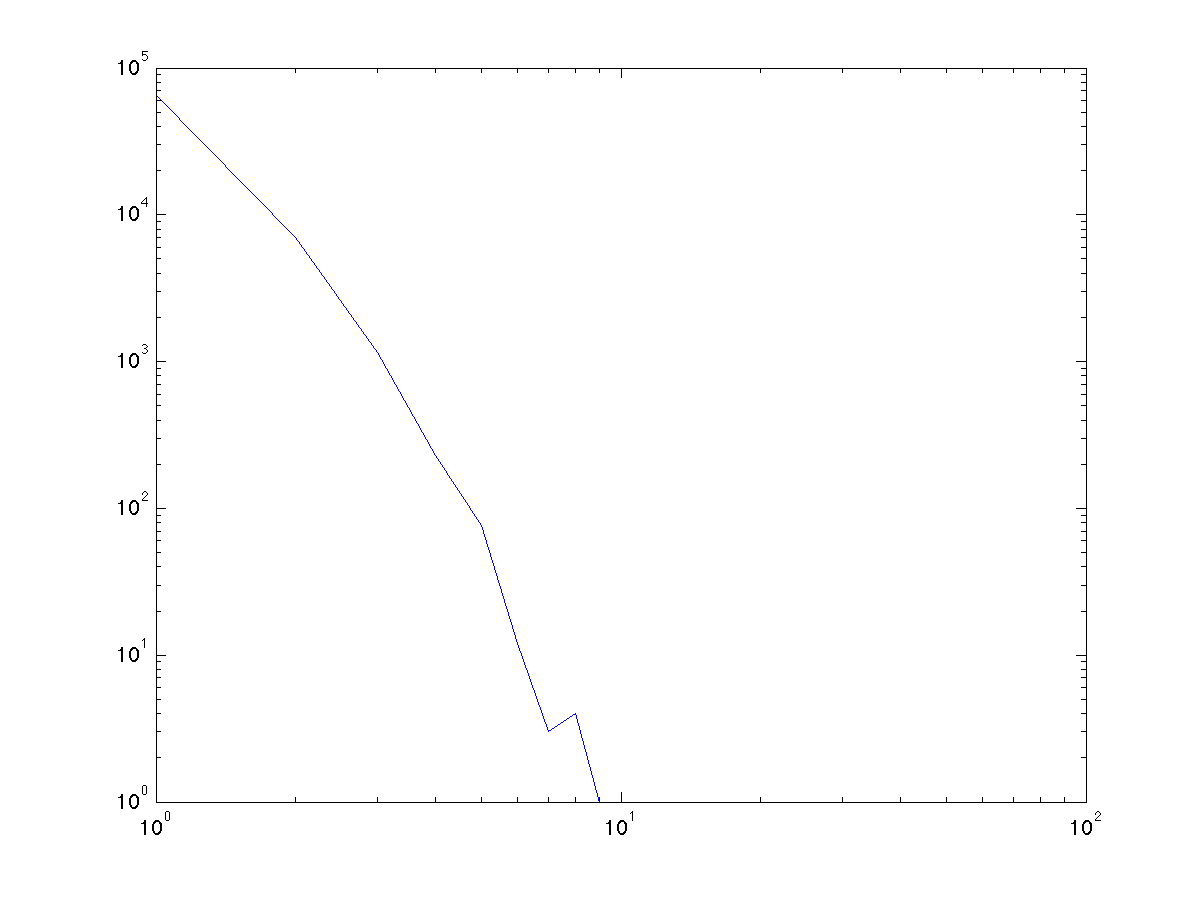
\includegraphics[width=.3\linewidth]{FIG/soc-pokec-75000.txt-indegreedist.png}}\hfill
\subfloat[Out-Degree Distribution\label{fig:soc-pokec_outdegree}]
  {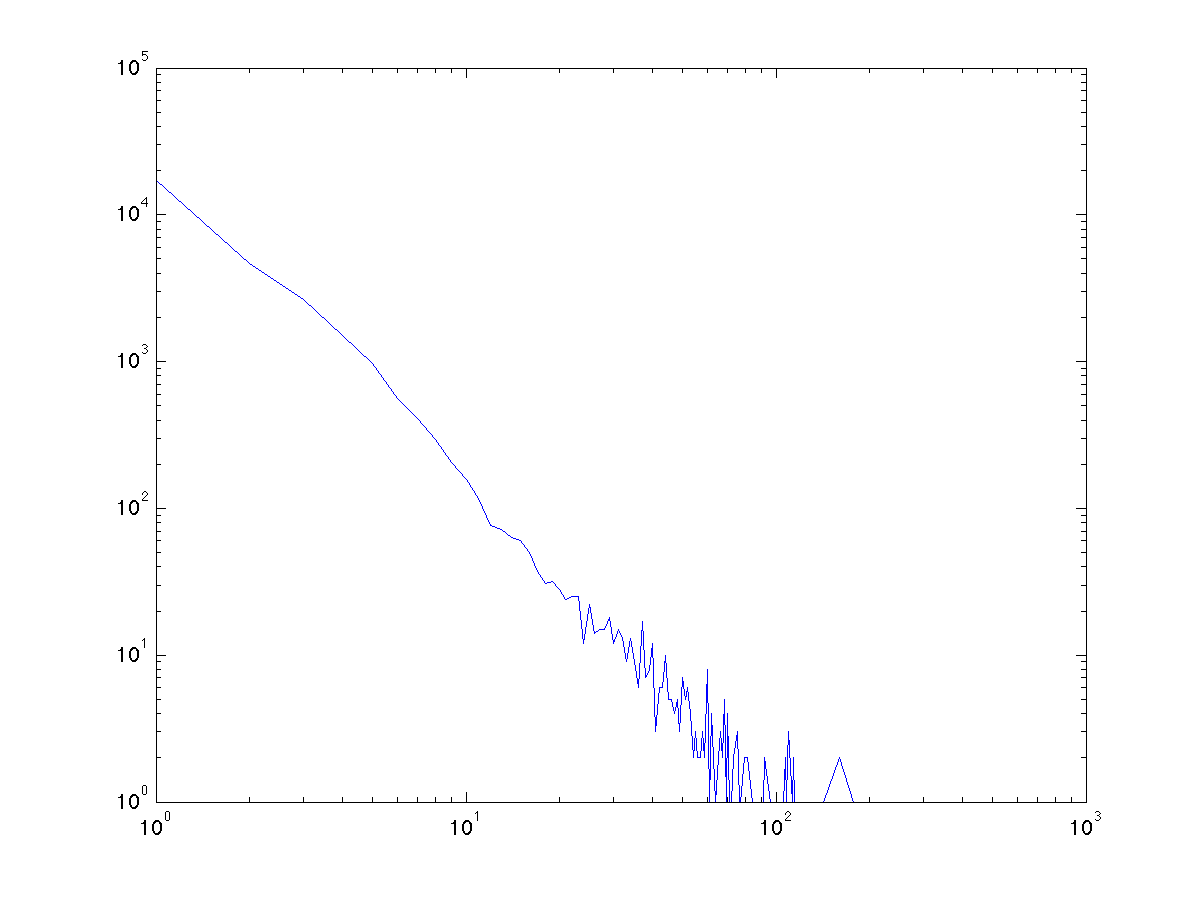
\includegraphics[width=.3\linewidth]{FIG/soc-pokec-75000.txt-outdegreedist.png}}\hfill
\subfloat[Degree Distribution\label{fig:soc-pokec_degree}]
  {\includegraphics[width=.3\linewidth]{FIG/soc-pokec-75000.txt-degree.png}}
\caption{Degree Distributions of soc-pokec\label{fig:soc-pokec_degree_dist}}
\end{figure}
\begin{figure}
\subfloat[In-Degree Distribution\label{fig:soc-Youtube_indegree}]
  {\includegraphics[width=.3\linewidth]{FIG/soc-Youtube-75000.undir.txt-indegreedist.png}}\hfill
\subfloat[Out-Degree Distribution\label{fig:soc-Youtube_outdegree}]
  {\includegraphics[width=.3\linewidth]{FIG/soc-Youtube-75000.undir.txt-outdegreedist.png}}\hfill
\subfloat[Degree Distribution\label{fig:soc-Youtube_degree}]
  {\includegraphics[width=.3\linewidth]{FIG/soc-Youtube-75000.undir.txt-degree.png}}
\caption{Degree Distributions of soc-Youtube\label{fig:soc-Youtube_degree_dist}}
\end{figure}

\clearpage

\begin{figure}
\subfloat[In-Degree Distribution\label{fig:soft-jdkdependency_indegree}]
  {\includegraphics[width=.3\linewidth]{FIG/soft-jdkdependency.txt-indegreedist.png}}\hfill
\subfloat[Out-Degree Distribution\label{fig:soft-jdkdependency_outdegree}]
  {\includegraphics[width=.3\linewidth]{FIG/soft-jdkdependency.txt-outdegreedist.png}}\hfill
\subfloat[Degree Distribution\label{fig:soft-jdkdependency_degree}]
  {\includegraphics[width=.3\linewidth]{FIG/soft-jdkdependency.txt-degree.png}}
\caption{Degree Distributions of soft-jdkdependency\label{fig:soft-jdkdependency_degree_dist}}
\end{figure}
\begin{figure}
\subfloat[In-Degree Distribution\label{fig:text-spanishbook_indegree}]
  {\includegraphics[width=.3\linewidth]{FIG/text-spanishbook.txt-indegreedist.png}}\hfill
\subfloat[Out-Degree Distribution\label{fig:text-spanishbook_outdegree}]
  {\includegraphics[width=.3\linewidth]{FIG/text-spanishbook.txt-outdegreedist.png}}\hfill
\subfloat[Degree Distribution\label{figt:ext-spanishbook_degree}]
  {\includegraphics[width=.3\linewidth]{FIG/text-spanishbook.txt-degree.png}}
\caption{Degree Distributions of text-spanishbook\label{fig:text-spanishbook_degree_dist}}
\end{figure}



\subsubsection{Weakly Connected Component and Triangle count}
\textbf{Global Pattern} \\
We find that most graphs consist of a small number of groups (compared with the total number of nodes). And most nodes are in one biggest groups. \\
And the triangle number illustrates how nodes in groups are connected to each other. \\
\\
\textbf{Strange Behaviors} \\
\begin{itemize} 
\item p2p-Gnutella31 has 12 components. This shows the nodes in this graph are highly connected. But the triangle count is little. So it seems that there are several popular nodes in this graph. And most nodes connect to these popular servers instead of connecting to each others. \\
\item cit-HepPh has 61 components and the triangle count is a large number. This shows the nodes in this graph are mostly connected to each others. \\
\item email-EuAll has 15836 components. Although the maximun component size is huge, the connections between nodes are not strong. It illustrates people are more likely to form small discussion groups in daily work communication.\\
\item ca-AstroPh and email-Enron have extremely high triangle counts. Which shows the nodes in these 2 graphs are very densely connected.\\
\item Nodes in as-Caida are all connected. And the triangles is much more than nodes number. Which indicates the graph is very dense. \\
\item Nodes in cit-Cora are also all connected. But the triangle number is not large compared with the nodes number. So this graph is more likely to be a star type graph (highly centralize).\\
\item In soc-hamsterster, triangles number is huge compared with members in each components. This shows that each components are highly connected. So the members in each components are very related with each other.\\
\item soc-pokec has extremely small triangles number(4.8). Which indicates the graph is highly centralize in each sub groups.\\
\item soft-jdkdependency and text-spanishbook both have large triangles numbers and all connected. The graphs are very dense. \\
\end{itemize} 
\scalebox{0.8}{
\begin{tabular}{| l | c | c | c | c | c |} \hline
\textbf{Metrics} & \textbf{as-skitter} & \textbf{ca-AstroPh} & \textbf{cit-HepPh} & \textbf{cit-HepTh} & \textbf{com-amazon} \\ \hline
components & 310 & 290 & 61 & 143 & 1946 \\ \hline
max group & 69768 & 17926 & 34454 & 27465 & 47556 \\ \hline
triangle & 28389.34144 & 1061822.808 & 60696.51906 & 191035.2798 & 132.7590596 \\ \hline
\end{tabular}}\\
\\
\\
\scalebox{0.8}{
\begin{tabular}{| l | c | c | c | c | c |} \hline
\textbf{Metrics} & \textbf{com-dblp} & \textbf{email-Enron} & \textbf{email-EuAll} & \textbf{p2p-Gnutella31} & \textbf{soc-Slashdot0811} \\ \hline
components & 949 & 1065 & 15836 & 12 & 2091\\ \hline
max group & 67361 & 33696 & 224832 & 62561 & 72780\\ \hline
triangle & 786.338039 & 2059367.367 & 370075.0779 & 307.5803753 & 252186.8962\\ \hline
\end{tabular}}\\
\\
\\
\scalebox{0.8}{
\begin{tabular}{| l | c | c | c | c | c |} \hline
\textbf{Metrics} & \textbf{as-Caida} & \textbf{bio-protein} & \textbf{cit-Cora} & \textbf{soc-digg} & \textbf{soc-flickr} \\ \hline
components & 1 & 173 & 1 & 373 & 1280 \\ \hline
max group & 26475 & 1458 & 23166 & 29652 & 63529 \\ \hline
triangle & 29967.0841542 & 30.1742701786 & 3192.44451312 & 5207.40905806 & 1574.17467495 \\ \hline
\end{tabular}}\\
\\
\\
\scalebox{0.8}{
\begin{tabular}{| l | c | c | c | c | c |} \hline
\textbf{Metrics} & \textbf{soc-hamsterster} & \textbf{soc-pokec} & \textbf{soc-Youtube} & \textbf{soft-jdkdependency} & \textbf{text-spanishbook} \\ \hline
components & 23 & 113 & 4319 & 1 & 1\\ \hline
max group & 1788 & 73564 & 54143 & 6434 & 12643\\ \hline
triangle & 15328.5846289 & 4.77180117934 & 100.71969417 & 150378.549887 & 191251.983102\\ \hline
\end{tabular}}\\

\subsubsection{PageRank}

\begin{figure}
\subfloat[as-skitter.75000\label{fig:as-skitter}]
  {\includegraphics[width=.25\linewidth]{FIG/pagerank/as-skitter_75000.png}}\hfill
\subfloat[ca-AstroPh\label{fig:ca-AstroPh}]
  {\includegraphics[width=.25\linewidth]{FIG/pagerank/ca-AstroPh.png}}\hfill
\subfloat[cit-HepPh\label{fig:cit-HepPh}]
  {\includegraphics[width=.25\linewidth]{FIG/pagerank/cit-HepPh.png}} \hfill
\subfloat[cit-HepTh\label{fig:cit-HepTh}]
  {\includegraphics[width=.25\linewidth]{FIG/pagerank/cit-HepTh.png}}\hfill
\subfloat[com-amazon.ungraph-75000\label{fig:com-amazon.ungraph-75000}]
  {\includegraphics[width=.25\linewidth]{FIG/pagerank/com-amazon.ungraph-75000.png}}\hfill
\subfloat[com-dblp.ungraph-75000\label{fig:com-dblp.ungraph-75000}]
  {\includegraphics[width=.25\linewidth]{FIG/pagerank/com-dblp.ungraph-75000.png}} \hfill
 \subfloat[email-Enron.ungraph\label{fig:email-Enron.ungraph}]
  {\includegraphics[width=.25\linewidth]{FIG/pagerank/email-Enron.ungraph.png}}\hfill
\subfloat[email-EuAll\label{fig:email-EuAll}]
  {\includegraphics[width=.25\linewidth]{FIG/pagerank/email-EuAll.png}}\hfill
\subfloat[p2p-Gnutella31\label{fig:p2p-Gnutella31}]
  {\includegraphics[width=.25\linewidth]{FIG/pagerank/p2p-Gnutella31.png}} \hfill
 \subfloat[soc-Slashdot0811-75000\label{fig:soc-Slashdot0811-75000}]
  {\includegraphics[width=.25\linewidth]{FIG/pagerank/soc-Slashdot0811-75000.png}} 
 \subfloat[as-Caida\label{fig:as-Caida}]
  {\includegraphics[width=.25\linewidth]{FIG/pagerank/as-Caida.undir.txt.png}} \hfill  
 \subfloat[bio-protein\label{fig:bio-protein}]
  {\includegraphics[width=.25\linewidth]{FIG/pagerank/bio-protein-undir.txt.png}} \hfill  
 \subfloat[cit-Cora\label{fig:cit-Cora}]
  {\includegraphics[width=.25\linewidth]{FIG/pagerank/cit-Cora.txt.png}} \hfill 
 \subfloat[soc-digg\label{fig:soc-digg}]
  {\includegraphics[width=.25\linewidth]{FIG/pagerank/soc-digg.txt.png}} \hfill  
 \subfloat[soc-flickr-75000\label{fig:soc-flickr-75000}]
  {\includegraphics[width=.25\linewidth]{FIG/pagerank/soc-flickr-75000.txt.png}} \hfill  
 \subfloat[soc-hamsterster\label{fig:soc-hamsterster}]
  {\includegraphics[width=.25\linewidth]{FIG/pagerank/soc-hamsterster.undir.txt.png}} \hfill  
 \subfloat[soc-pokec-75000\label{fig:soc-pokec-75000}]
  {\includegraphics[width=.25\linewidth]{FIG/pagerank/soc-pokec-75000.txt.png}} \hfill  
 \subfloat[soc-Youtube-75000\label{fig:soc-Youtube-75000}]
  {\includegraphics[width=.25\linewidth]{FIG/pagerank/soc-Youtube-75000.undir.txt.png}} \hfill  
 \subfloat[soft-jdkdependency\label{fig:soft-jdkdependency}]
  {\includegraphics[width=.25\linewidth]{FIG/pagerank/soft-jdkdependency.txt.png}} \hfill  
 \subfloat[text-spanishbook\label{fig:text-spanishbook}]
  {\includegraphics[width=.25\linewidth]{FIG/pagerank/text-spanishbook.txt.png}} \hfill  
\caption{Pagerank value Distributions of 20 graphs}
\label{fig:pagerank}
\end{figure}

To analyze the patterns of PageRank in 20 graphs, we calculated the PageRank value of nodes in each graphs, aggregated the values into distribution, and plotted the distribution in log-log scale. Mainly, we wanted to check whether the distribution of PageRank values follow power law or not. At the same time, we observed the charts of distribution to find out strange patterns of PageRank.
\\
\\
\textbf{Global Pattern}
\\
\\
The experiment result (Figure. \ref{fig:pagerank}) shows that the PageRank value distribution in most of graphs follow power law.
\\
\\
\textbf{Strange Behaviors}
\\
\\
(1) Plateau in the Beginning
\\
\\
The distribution of PageRank in most of graphs follow power low; however, we found that there are plateaus in the beginning part of some distribution charts. Taking com-amazon.ungraph-75000 for example, the line between $10^{-8}$ and $10^{-5}$ is relative smooth. 
\\
ca-AstroPh, com-amazon.ungraph-75000, com-dblp.ungraph-75000, email-Enron.ungraph, soc-Slashdot0811-75000, as-Caida, soc-flickr-75000, soc-pokec-75000, soc-Youtube-75000, and text-spanishbook have such plateau pattern.
\\
\\
(2) Broom Tail
\\
\\
Ideally, the chart of distribution following power law would be a smooth descending straight line in log-log scale plot; however, we found that some lines of real data are not as smooth as ideal straight lines. Instead, the lines of some real data jump up and down in the last part. The shape is like a bloom.
\\
as-skitter, cit-HepTh, email-Enron.ungraph, email-EuAll, as-Caida, cit-Cora, soc-Youtube-75000, soft-jdkdependency, and text-spanishbook have such broom tail pattern.
\\
\\
(3) Vibrating Line
\\
\\
The lines in PageRank distribution chart are usually smooth, but there are some lines vibrating severely. Taking soc-hamsterster for example, its line jumps up and down severely, although the trend of line follow power-law. bio-protein and soc-hamsterster have such pattern.



\subsubsection{Eigenvalue computation (via Lanczos-SO and QR algorithms)}

\begin{center}
\scalebox{0.6}{
  \begin{tabular}{ |l | c | c | c | c | c | c |  }
    \hline
      & \textbf{cit-HepPh} & \textbf{com-amazon.ungraph-75000}  & \textbf{com-dblp.ungraph-75000}  & \textbf{email-Enron.ungraph}  & \textbf{soc-Slashdot0811-75000}  \\ \hline
First Eigenvalue & 71.24869215  & 12.46375985 & 18.08047143  & 232.0718265 & 124.3376448  \\ \hline
Second Eigenvalue & 15.78100055 & -10.49450063 & -9.989018866 & -52.74314639 & -74.23852603  \\ \hline
Third Eigenvalue & -11.28234916 & 2.528983265  & 3.950839681 & 16.07981363 & 3.277331459  \\ \hline
  \end{tabular}}
\end{center}

\begin{center}
\scalebox{0.6}{
  \begin{tabular}{ |l | c | c | c | c | c | c |  }
    \hline
      & \textbf{p2p-Gnutella31} & \textbf{ca-AstroPh} & \textbf{email-EuAll} & \textbf{cit-HepTh} & \textbf{as-skitter.75000}\\ \hline
First Eigenvalue & 12.26069439 & 182.7509283 & 134.5445114 & 108.0148181 & 182.7509283 \\ \hline
Second Eigenvalue & 2.714800955 & 64.42806942 & -59.94291686 & -48.59746457 & 64.42806942 \\ \hline
Third Eigenvalue & -2.60170164 & -0.449525922 & 6.537952019 & 9.103275079 & -0.449525922 \\ \hline
  \end{tabular}}
\end{center}

\begin{center}
\scalebox{0.6}{
  \begin{tabular}{ |l | c | c | c | c | c | c |  }
    \hline
      & \textbf{as-Caida.undir} & \textbf{bio-protein-undir} & \textbf{cit-Cora} & \textbf{soc-digg} & \textbf{soc-flickr-75000}\\ \hline
First Eigenvalue & 68.3693197062366 & 6.59050522092269 & 27.0826721488691 & 31.4948560594139 & 46.128302835195 \\ \hline
Second Eigenvalue & -51.89780364579 & -4.73938936859157 & -9.39990749609768 & 3.5437520638839 & -44.5991249417485 \\ \hline
Third Eigenvalue & 0.336124325308012 & 1.07545809389524 & 4.9442935842295 & -3.43736182466055 & 1.53574108698456 \\ \hline
  \end{tabular}}
\end{center}

\begin{center}
\scalebox{0.6}{
  \begin{tabular}{ |l | c | c | c | c | c | c |  }
    \hline
      & \textbf{soc-hamsterster.undir} & \textbf{soc-pokec-75000} & \textbf{soc-Youtube-75000.undir} & \textbf{soft-jdkdependency} & \textbf{text-spanishbook}\\ \hline
First Eigenvalue & 45.2761211252026 & 9.38962714926706 & 15.7609882639711 & 143.265820052228 & 124.70922072648 \\ \hline
Second Eigenvalue & -10.0662421612482 & -9.28310856022425 & -14.9067351906316 & -126.79096036676 & -92.5441274101652 \\ \hline
Third Eigenvalue & 5.6332490229777 & 0.918759752366816 & 1.16658315444281 & 2.26001659190722 & 8.30033058289115 \\ \hline
  \end{tabular}}
\end{center}



\subsubsection{K-core algorithm}
To analyze K-core value, we set k = 5, applied K-core algorithm on 20 graphs, and counted the distribution of k-core size. We were curious about the patterns of the K-core size distribution. 
\\
\\
\textbf{Global Pattern}
\\
\\
According to the result, we found that the graphs can be grouped into two types of graphs: Type I graphs and Type II graphs.
\\
\\
\textbf{Type I Graphs}
\\
\\
Type I graphs, like soc-Slashdot0811-75000, p2p-Gnutella31, email-EuAll, email-Enron.ungraph, cit-HepTh, cit-HepPh, ca-AstroPh , as-Caida, cit-Cora, soc-digg, soc-flickr-75000, soc-hamsterster, soft-jdkdependency, and ca-AstroPh, have a giant 5-core with more than 1000 nodes, which means that type I graph is densely connected. 
\\
\\
\textbf{Type II Graphs}
\\
\\
Type II graphs, like as-skitter.75000, com-dblp.ungraph-75000, com-amazon.ungraph-75000, bio-protein, soc-pokec, and soc-Youtube-75000, do not have such a giant k-core. Instead, there are many small (size $<$ 500) 5-cores in type II graphs. Moreover, some graphs even do not have 5-cores, like bio-protein, soc-pokec, and soc-Youtube-75000. It indicates that Type II graphs are not densely connected.
\\
\begin{center}
\scalebox{0.6}{
  \begin{tabular}{ |c | c | c | c | c | c | c | c | c | c | c | c | c | c |  }
    \hline
         \multicolumn{2}{|c|}{soc-Slashdot0811-75000} & \multicolumn{2}{c|}{p2p-Gnutella31} & \multicolumn{2}{c|}{email-EuAll} & \multicolumn{2}{c|}{email-Enron.ungraph} & \multicolumn{2}{c|}{cit-HepTh} & \multicolumn{2}{c|}{cit-HepPh} & \multicolumn{2}{c|}{ca-AstroPh} \\ \hline
		size & frequency & size & frequency & size & frequency & size & frequency & size & frequency & size & frequency & size & frequency  \\ \hline
		26137  & 1 &16174  & 1 & 7030 & 1 & 6 & 6 & 21181 & 1 & 28593 & 1 & 6 & 2 \\ \hline
		& & & & & & 7 & 2 & & & & & 7 & 2 \\ \hline
		& & & & & & 8 & 3 & & & & & 8 & 1 \\ \hline
		& & & & & & 9 & 1 & & & & & 11 & 1 \\ \hline
		& & & & & & 12 & 1 & & & &  & 18 & 1 \\ \hline
		& & & & & & 15 & 1 & & & &  & 12236 & 1 \\ \hline
		& & & & & & 11538 & 1 & & & & &   &  \\ \hline
  \end{tabular}}
\scalebox{0.6}{
  \begin{tabular}{ |c | c | c | c | c | c | c | c | c | c | c | c | c | c |  }
    \hline
         \multicolumn{2}{|c|}{as-Caida} & \multicolumn{2}{c|}{cit-Cora} & \multicolumn{2}{c|}{soc-digg} & \multicolumn{2}{c|}{soc-flickr-75000} & \multicolumn{2}{c|}{soc-hamsterster} & \multicolumn{2}{c|}{soft-jdkdependency} & \multicolumn{2}{c|}{ca-AstroPh} \\ \hline
		size & frequency & size & frequency & size & frequency & size & frequency & size & frequency & size & frequency & size & frequency  \\ \hline
		1192  & 1 & 9355 & 1 & 6794 & 1 & 1122 & 1 & 1070 & 1 & 4869 & 1 & 3144 & 1 \\ \hline
		& & & & & & & & & & & & & \\ \hline
  \end{tabular}}  
  \\5-core distribution in Type I graphs
\end{center}

\begin{center}
\scalebox{0.6}{
  \begin{tabular}{ |c | c | c | c | c | c | c | c | c | c | c | c |  }
    \hline
         \multicolumn{2}{|c|}{as-skitter.75000} & \multicolumn{2}{c|}{com-dblp.ungraph-75000} & \multicolumn{2}{c|}{com-amazon.ungraph-75000} & \multicolumn{2}{c|}{bio-protein}  & \multicolumn{2}{c|}{soc-pokec}  & \multicolumn{2}{c|}{soc-Youtube-75000}  \\ \hline
		size & frequency & size & frequency & size & frequency & size & frequency & size & frequency & size & frequency   \\ \hline
		14  & 1 & 6 & 9 & 6 & 1 & 6 & 1 & 0 & 0 & 0 & 0 \\ \hline
		181 & 1 & 7 & 3 & & & & & & & &  \\ \hline
		& & 8 & 3 & & & & & & & & \\ \hline
		& & 9 & 1 & & & & & & & & \\ \hline
		& & 10 & 1 & & & & & & & & \\ \hline
		& & 13 & 1 & & & & & & & & \\ \hline
		& & 15 & 1 & & & & & & & & \\ \hline
  \end{tabular}}
    \\5-core distribution in Type II graphs
\end{center}


	
\section{Division of Labour}
	\label{sec:dl}
    \begin{itemize*}
\item
Jiajung Wang: 

\begin{itemize*}
\item
Degree Distribution analysis
\item
Weakly Connected Component analysis
\item
Triangle count analysis
\item
Organize latex files
\end{itemize*}

\item
San-Chuan Hung: 

\begin{itemize*}
\item 
PageRank analysis
\item 
K-core analysis
\item
Eigenvalue analysis
\item
Organize latex files
\end{itemize*}
\end{itemize*}

	
\bibliography{BIB/sanchuah}
\bibliographystyle{plain}

\end{document}
